%************************************************
\chapter{Modelling hippocampal place cells for visual localization}\label{ch:chapter5} % 
%************************************************


\section{Introduction}


Place cells are a special type of neurons located in the hippocampus which fire when an animal ``recognises'' a particular place in the environment. These cells were discovered by John O'Keefe, and together with Edvard and May-Britt Moser for their discovery of grid cells received the 2014 Nobel Prize in Physiology or Medicine. This award highlights the importance of the discovery,let alone because these cells are located in one of the least known but more attractive areas of our brains: the hippocampus, with a key role in memory.

\section{Biological background}

\subsection{Place cells}

\subsubsection{Place fields}

\subsubsection{Cognitive map}

\subsubsection{Misplace cells}

\subsection{Allocentric representation}

\subsection{Sensory input}

\subsubsection{Metric vs contextual}

\subsubsection{Visuospatial cues}

\subsection{Population encoding}

\section{Modelling a single place cell}

We refer to place cells, according to the previous section, as a biological term to denominate a special type of neurons sensitive to specific spatial locations. This point forward, the term ``place cell'' will also be used not only to describe a biological entity but to refer to the output of a series of algorithms that mimic the behaviour of their biological counterparts.

Given the nature of image matching techniques, one would expect high scores when two images are visually similar, and low ones when they are dissimilar. 

%Additionally, as the visual paths datasets analysed in this work present a sequential

If we take an unseen query frame from one of the passes of the RSM dataset and use one of the similarty metrics described in Section \ref{sec:metrics}


\section{Results}

\begin{figure}
	\centering
	\setlength\figureheight{0.6\textwidth}
	\setlength\figurewidth{0.8\textwidth}
		% This file was created by matlab2tikz.
% Minimal pgfplots version: 1.3
%
%The latest updates can be retrieved from
%  http://www.mathworks.com/matlabcentral/fileexchange/22022-matlab2tikz
%where you can also make suggestions and rate matlab2tikz.
%
\definecolor{mycolor1}{rgb}{0.00000,0.44700,0.74100}%
%
\begin{tikzpicture}

\begin{axis}[%
width=0.95092\figurewidth,
height=\figureheight,
at={(0\figurewidth,0\figureheight)},
scale only axis,
xmin=517,
xmax=816,
xlabel={Frame index},
ymin=1.79650837845272,
ymax=7.37640317281087,
ylabel={$\chi{}^\text{2}\text{ score}$}
]
\addplot [color=mycolor1,solid,line width=2.0pt,forget plot]
  table[row sep=crcr]{%
517	5.45564129617479\\
518	5.28480574819777\\
519	5.38022258546617\\
520	5.04640165964762\\
521	4.91818147235447\\
522	5.02140005429586\\
523	4.9060054090288\\
524	5.14407377772861\\
525	4.78613996505737\\
526	4.74626959694756\\
527	4.60538254843818\\
528	4.73193724950155\\
529	4.89160471492344\\
530	4.61402278476291\\
531	4.74068803257412\\
532	4.82834929890103\\
533	4.78515206442939\\
534	5.00995551215278\\
535	4.93059447076586\\
536	4.747631099489\\
537	4.85051237212287\\
538	4.85323116514418\\
539	4.79317005475362\\
540	4.78844994968838\\
541	4.7296888033549\\
542	4.57528159353468\\
543	4.6541080739763\\
544	4.73621863789029\\
545	4.60128768285116\\
546	4.72721687952677\\
547	4.7022082540724\\
548	4.51559209823608\\
549	4.45021396213108\\
550	4.61597768465678\\
551	4.58577950795492\\
552	4.56056160397\\
553	4.61316866344876\\
554	4.44940259721544\\
555	4.33124679989285\\
556	4.31974034839206\\
557	4.24667429924011\\
558	4.18328481250339\\
559	4.32105019357469\\
560	4.36144169171651\\
561	4.33154243893093\\
562	4.2965227233039\\
563	4.45881326993306\\
564	4.60404780175951\\
565	4.9832649230957\\
566	5.21849367353651\\
567	5.42206896675958\\
568	5.61464606391059\\
569	5.32002242406209\\
570	5.31870725419786\\
571	5.20021793577406\\
572	5.55876763661702\\
573	5.52424425548977\\
574	5.40127817789714\\
575	5.50023322635227\\
576	5.73416566848755\\
577	5.55387417475383\\
578	5.5627646446228\\
579	5.47471041149563\\
580	5.35248724619548\\
581	4.86793337927924\\
582	4.91971654362149\\
583	4.92856052186754\\
584	5.1939090622796\\
585	4.77915970484416\\
586	4.61318797535366\\
587	4.59124125374688\\
588	4.83357630835639\\
589	4.78117969301012\\
590	4.8751319249471\\
591	5.01082160737779\\
592	5.23354652192858\\
593	4.6385703086853\\
594	4.53041002485487\\
595	4.51224210527208\\
596	4.43363348642985\\
597	4.25946267445882\\
598	4.22609305381775\\
599	4.34774973657396\\
600	4.57303765085008\\
601	4.32682673136393\\
602	4.77783237563239\\
603	4.9052480061849\\
604	4.89262798097399\\
605	4.71505321396722\\
606	4.99992277887132\\
607	4.91769223743015\\
608	4.94722530576918\\
609	5.03998618655735\\
610	4.98740741941664\\
611	5.11870463689168\\
612	5.16300662358602\\
613	5.19595686594645\\
614	5.05345845222473\\
615	4.81346085336473\\
616	4.98365359836155\\
617	5.10461118486193\\
618	5.3875585132175\\
619	5.45500458611382\\
620	5.10809373855591\\
621	5.40080017513699\\
622	5.12411006291707\\
623	5.11253976821899\\
624	5.29478883743286\\
625	5.38006231519911\\
626	5.26761012607151\\
627	5.07983054055108\\
628	4.79844037691752\\
629	4.7360757721795\\
630	4.55040812492371\\
631	4.55683490965101\\
632	4.32798796229892\\
633	4.38316342565748\\
634	4.57085434595744\\
635	4.71197700500488\\
636	5.20676475101047\\
637	5.29618379804823\\
638	5.53390868504842\\
639	5.37041934331258\\
640	5.56473557154338\\
641	5.70307895872328\\
642	5.30179659525553\\
643	5.38066954082913\\
644	5.54609791437785\\
645	5.42192618052165\\
646	5.84239138497247\\
647	5.49786647160848\\
648	5.54475773705377\\
649	5.51714981926812\\
650	5.45711406071981\\
651	5.44256104363336\\
652	5.12285571628147\\
653	5.11807007259793\\
654	5.33797539605035\\
655	5.66756502787272\\
656	5.50892194112142\\
657	5.86675696902805\\
658	5.8700491587321\\
659	5.71904346677992\\
660	5.90887721379598\\
661	6.13676097657945\\
662	6.19742769665188\\
663	6.42192517386542\\
664	6.30267741945055\\
665	6.34279457728068\\
666	6.27500221464369\\
667	6.28113868501451\\
668	6.38645627763536\\
669	6.43902895185682\\
670	6.78609715567695\\
671	6.9065891901652\\
672	6.71403990851508\\
673	6.70098299450344\\
674	6.66558986239963\\
675	6.7139032681783\\
676	6.78372716903687\\
677	6.76429753833347\\
678	7.00557661056519\\
679	6.82014653417799\\
680	7.00547329584758\\
681	7.34336815940009\\
682	7.20823060141669\\
683	6.99682813220554\\
684	7.24651824103461\\
685	7.23865800433689\\
686	7.34053574668037\\
687	7.34751473532783\\
688	7.37640317281087\\
689	7.37493318981594\\
690	7.32039319144355\\
691	7.26464568244086\\
692	7.08425818549262\\
693	6.96295788553026\\
694	6.90606005986532\\
695	7.08241897159153\\
696	6.66772707303365\\
697	6.62142117818197\\
698	6.64435042275323\\
699	6.69112764464484\\
700	6.59604427549574\\
701	6.51153024037679\\
702	6.47479195064968\\
703	6.78648434744941\\
704	6.22314156426324\\
705	5.96851372718811\\
706	6.07606569925944\\
707	6.0125810570187\\
708	6.13718112309774\\
709	6.05301419893901\\
710	5.86252167489794\\
711	5.8945533964369\\
712	5.94143915176392\\
713	5.79714462492201\\
714	5.77606577343411\\
715	5.80971254242791\\
716	5.595112880071\\
717	5.6970772213406\\
718	5.93423128128052\\
719	5.84677373038398\\
720	5.82072750727336\\
721	5.70003567801581\\
722	5.5985779232449\\
723	5.41437101364136\\
724	5.41969439718458\\
725	5.26762652397156\\
726	5.31281068589952\\
727	5.33975100517273\\
728	5.22491206063165\\
729	5.03604883617825\\
730	5.22387671470642\\
731	5.00555160310533\\
732	4.94978168275621\\
733	4.51597449514601\\
734	4.7652227083842\\
735	4.92013684908549\\
736	4.85085704591539\\
737	4.84549196561178\\
738	4.6559042930603\\
739	4.86927668253581\\
740	4.71941457854377\\
741	4.81414641274346\\
742	4.79970055156284\\
743	4.69480657577515\\
744	4.71684855884976\\
745	4.59916199578179\\
746	4.60451703601413\\
747	4.55340411927965\\
748	4.76788369814555\\
749	4.70615172386169\\
750	4.6492067972819\\
751	4.7372952832116\\
752	4.70831603474087\\
753	4.95494400130378\\
754	4.93097477489048\\
755	5.05009076330397\\
756	4.83696320321825\\
757	4.65081408288744\\
758	4.9603201813168\\
759	5.27593053711785\\
760	5.34850931167603\\
761	5.34796449873182\\
762	5.31409517923991\\
763	5.15496057934231\\
764	5.20180945926242\\
765	5.18936035368178\\
766	4.8254066573249\\
767	5.08930932150947\\
768	4.86718906296624\\
769	4.62061770757039\\
770	4.98884542783101\\
771	5.15281282530891\\
772	5.03079618348016\\
773	4.79297688272264\\
774	4.88556533389621\\
775	5.0670190387302\\
776	4.6277256541782\\
777	4.46976200739543\\
778	4.50152950816684\\
779	4.35459629694621\\
780	4.15776922967699\\
781	4.18754514058431\\
782	4.16014623641968\\
783	4.23905968666077\\
784	4.11976922882928\\
785	3.84921227561103\\
786	4.09121913380093\\
787	4.26308623949687\\
788	3.93736775716146\\
789	4.12939588228862\\
790	4.14773575464884\\
791	4.02434510654873\\
792	3.93602151340908\\
793	3.89979214138455\\
794	3.81887470351325\\
795	3.75678775045607\\
796	3.81119052569071\\
797	3.97538926866319\\
798	3.73644529448615\\
799	3.62051859166887\\
800	3.63900767432319\\
801	3.4945670498742\\
802	3.44758110576206\\
803	3.41365891032749\\
804	3.53506263097127\\
805	3.68221312099033\\
806	3.50561817487081\\
807	3.18562004301283\\
808	2.92959801355998\\
809	2.77806928422716\\
810	2.53599411911435\\
811	2.5533709526062\\
812	2.44258156087663\\
813	2.23334169387817\\
814	1.9372197786967\\
815	1.97369148996141\\
816	1.79650837845272\\
};
\end{axis}
\end{tikzpicture}%
	\caption{Single tuning curve without smoothing}
\end{figure}

\begin{figure}
	\centering
	\setlength\figureheight{0.6\textwidth}
	\setlength\figurewidth{0.8\textwidth}
		% This file was created by matlab2tikz.
% Minimal pgfplots version: 1.3
%
%The latest updates can be retrieved from
%  http://www.mathworks.com/matlabcentral/fileexchange/22022-matlab2tikz
%where you can also make suggestions and rate matlab2tikz.
%
\definecolor{mycolor1}{rgb}{0.00000,0.44700,0.74100}%
%
\begin{tikzpicture}

\begin{axis}[%
width=0.95092\figurewidth,
height=\figureheight,
at={(0\figurewidth,0\figureheight)},
scale only axis,
xmin=517,
xmax=816,
xlabel={Frame index},
ymin=1.79650837845272,
ymax=6.71851701963516,
ylabel={$\chi{}^\text{2}\text{ score}$}
]
\addplot [color=mycolor1,solid,line width=2.0pt,forget plot]
  table[row sep=crcr]{%
517	5.45564129617479\\
518	5.37355654327958\\
519	5.21705055236816\\
520	5.14466546073792\\
521	5.10476355199461\\
522	5.02677491939429\\
523	4.99369739059709\\
524	4.95151845967328\\
525	4.93448695637821\\
526	4.9382541179657\\
527	4.9249986529981\\
528	4.91614664925469\\
529	4.90358046743605\\
530	4.88218153160786\\
531	4.86746233359151\\
532	4.85760750992751\\
533	4.83489814751879\\
534	4.82152560173519\\
535	4.80884125211217\\
536	4.78737886475022\\
537	4.76278513104612\\
538	4.73903547392951\\
539	4.7215891002137\\
540	4.70695415963518\\
541	4.71049302505528\\
542	4.7056532776545\\
543	4.70845456782923\\
544	4.71323872045054\\
545	4.71882281768349\\
546	4.72699681323131\\
547	4.73064615775128\\
548	4.74396783586532\\
549	4.75172641704412\\
550	4.76428025812248\\
551	4.77966727096748\\
552	4.80270366117257\\
553	4.8194778841369\\
554	4.83317502555933\\
555	4.85074007916613\\
556	4.8632257774033\\
557	4.86403361577836\\
558	4.86677982963942\\
559	4.86511870738871\\
560	4.87049247456246\\
561	4.87113591548807\\
562	4.86629256045197\\
563	4.86094582756631\\
564	4.86177044498677\\
565	4.8616220724015\\
566	4.86459029937277\\
567	4.87347887108385\\
568	4.88530414553186\\
569	4.88331132248686\\
570	4.88186483967061\\
571	4.8774775993797\\
572	4.87199648167271\\
573	4.86676935057521\\
574	4.86219545448719\\
575	4.85672141473039\\
576	4.85646137683029\\
577	4.85169127738935\\
578	4.85505176131147\\
579	4.86435472884146\\
580	4.87581148763903\\
581	4.88387909714056\\
582	4.89925151509222\\
583	4.91423942172338\\
584	4.92701850564572\\
585	4.9408663524792\\
586	4.95425135208095\\
587	4.97103057480723\\
588	4.98540186773893\\
589	4.99748164455907\\
590	4.9989141655617\\
591	4.99064818963983\\
592	4.98170093722354\\
593	4.97129206214092\\
594	4.9726703496747\\
595	4.97545192787707\\
596	4.97357184221955\\
597	4.97034801647506\\
598	4.96218201254501\\
599	4.95628939193933\\
600	4.95209664930832\\
601	4.94487005026162\\
602	4.93902792681912\\
603	4.92917212877684\\
604	4.91537069949974\\
605	4.90279087349941\\
606	4.89631076626767\\
607	4.88890501863562\\
608	4.87664843578728\\
609	4.86010260646846\\
610	4.85585147669526\\
611	4.85786757934121\\
612	4.87042928336699\\
613	4.87987025254438\\
614	4.89523206870842\\
615	4.90533997520568\\
616	4.9166443418213\\
617	4.92622663644977\\
618	4.93976186678793\\
619	4.95711410180782\\
620	4.97821319995283\\
621	4.99838243860777\\
622	5.03068710616927\\
623	5.05664166571602\\
624	5.08107040041969\\
625	5.10033799569353\\
626	5.12340508404773\\
627	5.13697097523142\\
628	5.14141194890686\\
629	5.14601280791959\\
630	5.15872550551313\\
631	5.17235085753356\\
632	5.1844167698538\\
633	5.2031827221652\\
634	5.22012278282183\\
635	5.2350541307272\\
636	5.25118010168443\\
637	5.27105263950062\\
638	5.2914908197191\\
639	5.31941871199748\\
640	5.34981088681556\\
641	5.37754845781391\\
642	5.40143398903395\\
643	5.41967031907062\\
644	5.43867953726494\\
645	5.46584148039353\\
646	5.49411284734332\\
647	5.5304899723892\\
648	5.56317364872178\\
649	5.59187148866199\\
650	5.61810674472731\\
651	5.64762293130092\\
652	5.68239633188226\\
653	5.72251586578871\\
654	5.76883220942923\\
655	5.81515340145483\\
656	5.86512561341802\\
657	5.92666398478744\\
658	5.98431841694579\\
659	6.03382808605289\\
660	6.08555341740044\\
661	6.127020626652\\
662	6.16874209499143\\
663	6.20575446336448\\
664	6.24669290886444\\
665	6.28363571740062\\
666	6.31664213031328\\
667	6.35670027494971\\
668	6.39146739014693\\
669	6.42038289976228\\
670	6.4506713462795\\
671	6.4759780317207\\
672	6.49985273787224\\
673	6.52182546116057\\
674	6.54482955510925\\
675	6.57001350580159\\
676	6.59355397992123\\
677	6.62189427633134\\
678	6.64958247792424\\
679	6.67914388509565\\
680	6.69048218175668\\
681	6.69986160596212\\
682	6.70413321270153\\
683	6.70704202695228\\
684	6.71557544850979\\
685	6.71851701963516\\
686	6.71292029919268\\
687	6.70673919102502\\
688	6.69693335383928\\
689	6.68661635803257\\
690	6.67505046407652\\
691	6.66555475648028\\
692	6.65155422984878\\
693	6.63748526951623\\
694	6.62718327623916\\
695	6.60801341041686\\
696	6.58585296790886\\
697	6.56515900402112\\
698	6.54266094134238\\
699	6.51712586279629\\
700	6.49071343685764\\
701	6.45977260736652\\
702	6.4301504267046\\
703	6.39615398577822\\
704	6.36359818019564\\
705	6.32340584428403\\
706	6.2801509168413\\
707	6.2351982842227\\
708	6.19342182607067\\
709	6.13769644350151\\
710	6.08721817215554\\
711	6.03782227628626\\
712	5.98687007854315\\
713	5.93521882941664\\
714	5.87972844376856\\
715	5.82970565787248\\
716	5.77776216595622\\
717	5.73143335426746\\
718	5.68728524541098\\
719	5.64215762328669\\
720	5.59388067608788\\
721	5.55166506226641\\
722	5.51050375324258\\
723	5.4678313797023\\
724	5.42858150324313\\
725	5.3900122674955\\
726	5.35200566661601\\
727	5.31654655095401\\
728	5.27413495273547\\
729	5.24825336981793\\
730	5.22707910548532\\
731	5.20614084148623\\
732	5.18214864038826\\
733	5.15181461915948\\
734	5.12951474124882\\
735	5.11754349353903\\
736	5.10639973670717\\
737	5.09428800909427\\
738	5.08442985714158\\
739	5.07175424093562\\
740	5.0593480555649\\
741	5.05106739176103\\
742	5.03327819657704\\
743	5.01603489127559\\
744	4.99604336745074\\
745	4.97155133072211\\
746	4.95703724398364\\
747	4.94793999708699\\
748	4.9401119393286\\
749	4.92732178597223\\
750	4.91952461882784\\
751	4.91450846276316\\
752	4.89997733315102\\
753	4.88456610757477\\
754	4.87365754986025\\
755	4.85591713317127\\
756	4.8386154520809\\
757	4.82305960428147\\
758	4.81579780308297\\
759	4.80505978223148\\
760	4.78872574916502\\
761	4.76828401915881\\
762	4.75289069606063\\
763	4.74487400108995\\
764	4.72585545159251\\
765	4.71381425370975\\
766	4.70021403619762\\
767	4.68439045568713\\
768	4.66890504625108\\
769	4.65223042548649\\
770	4.63630619503203\\
771	4.61900559736758\\
772	4.60385838117189\\
773	4.58768502546816\\
774	4.56789509833805\\
775	4.54690146148881\\
776	4.52448742865435\\
777	4.49971704120809\\
778	4.46895453313581\\
779	4.43798890324677\\
780	4.40706996177059\\
781	4.38350363356186\\
782	4.36013228850029\\
783	4.32391391833083\\
784	4.27602958111536\\
785	4.22357162137151\\
786	4.16618447076707\\
787	4.10984316001944\\
788	4.0544884861732\\
789	3.99390751136944\\
790	3.92753729555342\\
791	3.86933902683171\\
792	3.80213900758566\\
793	3.76206392768427\\
794	3.70389658551157\\
795	3.64771100655391\\
796	3.58290216851687\\
797	3.533371826862\\
798	3.48501014709473\\
799	3.44571603063553\\
800	3.400025913611\\
801	3.36231850466848\\
802	3.30612304384224\\
803	3.25225202340648\\
804	3.1855489508311\\
805	3.12186565721668\\
806	3.05844036485783\\
807	2.97056146671897\\
808	2.88727670479444\\
809	2.79667528382054\\
810	2.69914532624758\\
811	2.53378304447791\\
812	2.35337503015259\\
813	2.21038685336946\\
814	2.07666858037313\\
815	1.90247321570361\\
816	1.79650837845272\\
};
\end{axis}
\end{tikzpicture}%
	\caption{Single tuning curve without smoothing}
\end{figure}

\subsection{Features of a place cell}

\begin{figure}
\centering
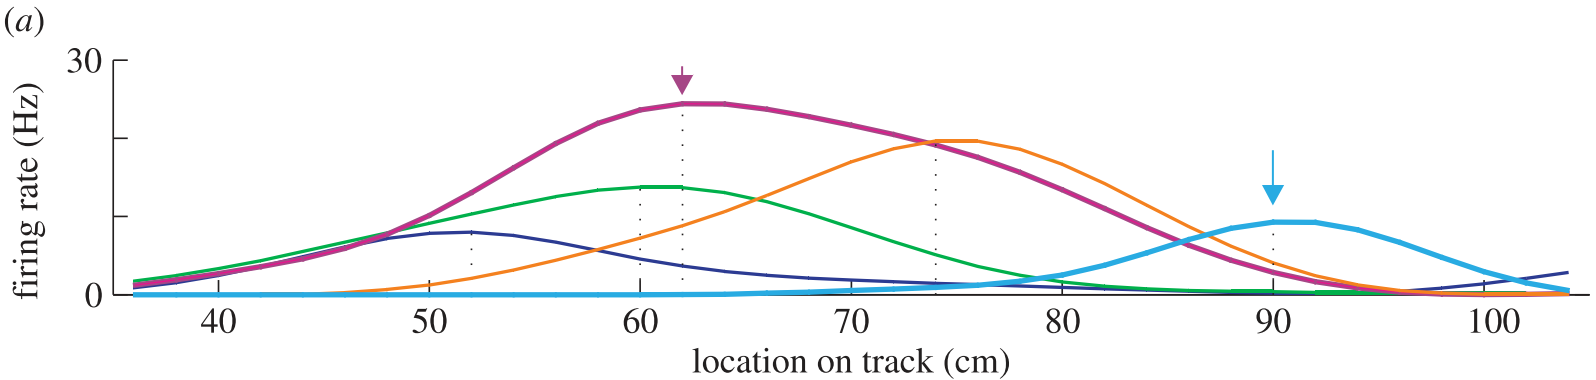
\includegraphics[width=\textwidth]{./gfx/Chapter05/dragoi_et_al_place_cell.png}
\caption{Caption}
\label{}
\end{figure}

\section{Modelling a place field}



% This file was created by matlab2tikz.
% Minimal pgfplots version: 1.3
%
%The latest updates can be retrieved from
%  http://www.mathworks.com/matlabcentral/fileexchange/22022-matlab2tikz
%where you can also make suggestions and rate matlab2tikz.
%
\definecolor{mycolor1}{rgb}{0.00000,0.44700,0.74100}%
\definecolor{mycolor2}{rgb}{0.85000,0.32500,0.09800}%
\definecolor{mycolor3}{rgb}{0.92900,0.69400,0.12500}%
\definecolor{mycolor4}{rgb}{0.49400,0.18400,0.55600}%
\definecolor{mycolor5}{rgb}{0.46600,0.67400,0.18800}%
\definecolor{mycolor6}{rgb}{0.30100,0.74500,0.93300}%
\definecolor{mycolor7}{rgb}{0.63500,0.07800,0.18400}%
%
\begin{tikzpicture}

\begin{axis}[%
width=\figurewidth,
height=\figureheight,
%at={(0.758333in,0.48125in)},
scale only axis,
xmin=-1193.72122445853,
xmax=1199.71982357641,
xlabel={Target: shifted ground truth location (cm)},
ymin=6,
ymax=16.9407386779785,
ylabel={Thresholded $\chi^2$ score.},
title style={font=\bfseries},
%title={},
axis x line*=bottom,
axis y line*=left,
legend style={legend cell align=left,align=left,at={(1.15,1)},draw=white!15!black}
]
\addplot [color=mycolor1,solid,line width=1.5pt]
  table[row sep=crcr]{%
-1193.72122445853	16.9407386779785\\
-1187.72262534064	15.6843627293905\\
-1181.72402622276	15.2515630722046\\
-1175.72542710488	14.9613719667707\\
-1169.726827987	14.5209669537014\\
-1163.72822886912	14.0880492817272\\
-1157.72962975123	13.7599135912382\\
-1151.73103063335	13.4953484217326\\
-1145.73243151547	13.1921173544491\\
-1139.73383239759	12.8910260451467\\
-1133.73523327971	12.5336408615112\\
-1127.73663416182	12.258525497035\\
-1121.73803504394	11.9852022371794\\
-1115.73943592606	11.7476778532329\\
-1109.74083680818	11.500297847547\\
-1103.7422376903	11.2994679902729\\
-1097.74363857241	11.0807148280897\\
-1091.74503945453	10.9028805682534\\
-1085.74644033665	10.7555287511725\\
-1079.74784121877	10.6352120951602\\
-1073.74924210089	10.5394358383982\\
-1067.750642983	10.4399944104646\\
-1061.75204386512	10.3081314689235\\
-1055.75344474724	10.1789315876208\\
-1049.75484562936	10.0691849056043\\
-1043.75624651148	9.99731129094174\\
-1037.75764739359	9.94793906964754\\
-1031.75904827571	9.92680163132517\\
-1025.76044915783	9.90567262549149\\
-1019.76185003995	9.89353661788137\\
-1013.76325092207	9.87450092717221\\
-1007.76465180418	9.85822687650982\\
-1001.7660526863	9.82285986448589\\
-995.767453568419	9.79963829642848\\
-989.768854450537	9.75731101788972\\
-983.770255332655	9.71796648125899\\
-977.771656214773	9.70153080789666\\
-971.773057096891	9.70624391656173\\
-965.774457979009	9.68029463918585\\
-959.775858861127	9.61910006874486\\
-953.777259743245	9.55090447476035\\
-947.778660625363	9.5083128778558\\
-941.780061507481	9.48164021341424\\
-935.781462389599	9.45037073838083\\
-929.782863271716	9.46973976336027\\
-923.784264153834	9.47496559745387\\
-917.785665035952	9.48131757033499\\
-911.78706591807	9.50782745762875\\
-905.788466800188	9.50184606250964\\
-899.789867682306	9.50906507592452\\
-893.791268564424	9.52369484148527\\
-887.792669446542	9.53914873223555\\
-881.79407032866	9.56453002126593\\
-875.795471210778	9.5490964588366\\
-869.796872092896	9.56866088666414\\
-863.798272975014	9.57917951282702\\
-857.799673857132	9.57490228351794\\
-851.80107473925	9.59033870697021\\
-845.802475621368	9.64775732943886\\
-839.803876503486	9.69510218971654\\
-833.805277385604	9.74842136784604\\
-827.806678267722	9.77508474651136\\
-821.80807914984	9.78608422530325\\
-815.809480031958	9.75724431088096\\
-809.810880914076	9.71628364763762\\
-803.812281796194	9.66527768185264\\
-797.813682678312	9.59674433657998\\
-791.81508356043	9.58135007557116\\
-785.816484442548	9.51420804073936\\
-779.817885324665	9.42849480478387\\
-773.819286206784	9.38508691285786\\
-767.820687088901	9.3195642672087\\
-761.822087971019	9.30285905536852\\
-755.823488853137	9.25530378442062\\
-749.824889735255	9.22656907533345\\
-743.826290617373	9.21548763074373\\
-737.827691499491	9.18925717002467\\
-731.829092381609	9.16857940272281\\
-725.830493263727	9.17328488199334\\
-719.831894145845	9.15506603843287\\
-713.833295027963	9.15491746601306\\
-707.834695910081	9.15044674120451\\
-701.836096792199	9.12875080108643\\
-695.837497674317	9.11097682149787\\
-689.838898556435	9.12068894034938\\
-683.840299438553	9.14774287374396\\
-677.841700320671	9.14443568179482\\
-671.843101202789	9.21245404293662\\
-665.844502084907	9.25902431889584\\
-659.845902967025	9.2796664488943\\
-653.847303849143	9.30741144481458\\
-647.848704731261	9.31202692734568\\
-641.850105613379	9.27061116067987\\
-635.851506495497	9.19576165550633\\
-629.852907377614	9.13512101926302\\
-623.854308259732	9.09386200653879\\
-617.85570914185	9.04144299657721\\
-611.857110023968	9.01009637431094\\
-605.858510906086	8.99524535630879\\
-599.859911788204	8.98515979867233\\
-593.861312670322	8.96430123479743\\
-587.86271355244	8.97450022948416\\
-581.864114434558	8.99513623588964\\
-575.865515316676	8.98986151343898\\
-569.866916198794	8.96746858797575\\
-563.868317080912	8.94336858548616\\
-557.86971796303	8.90885536294235\\
-551.871118845148	8.89461991661473\\
-545.872519727266	8.85185625678615\\
-539.873920609384	8.80509660118505\\
-533.875321491502	8.77622290661461\\
-527.87672237362	8.75422299535651\\
-521.878123255738	8.81455496737832\\
-515.879524137856	8.86164755570261\\
-509.880925019974	8.88624115994102\\
-503.882325902091	8.91184079019647\\
-497.88372678421	8.90392454046952\\
-491.885127666327	8.89473202354029\\
-485.886528548445	8.89292059446636\\
-479.887929430563	8.90409394314414\\
-473.889330312682	8.88552675749126\\
-467.890731194799	8.85545795842221\\
-461.892132076917	8.83008414820621\\
-455.893532959035	8.79158416547273\\
-449.894933841153	8.75964189830579\\
-443.896334723271	8.70555571505898\\
-437.897735605389	8.68723251945094\\
-431.899136487507	8.6613833276849\\
-425.900537369625	8.66857950310958\\
-419.901938251743	8.6453625528436\\
-413.903339133861	8.64757530312789\\
-407.904740015979	8.60468194359227\\
-401.906140898097	8.52794564397711\\
-395.907541780215	8.44520601473356\\
-389.908942662333	8.37650778419093\\
-383.910343544451	8.30070821862472\\
-377.911744426569	8.23591817052741\\
-371.913145308687	8.12273103312442\\
-365.914546190805	7.99770124335038\\
-359.915947072923	7.90073911767257\\
-353.917347955041	7.81033402995059\\
-347.918748837159	7.73379142660844\\
-341.920149719277	7.65095959211651\\
-335.921550601395	7.58865281155235\\
-329.922951483512	7.54740172938297\\
-323.92435236563	7.49370165875084\\
-317.925753247748	7.46047298531783\\
-311.927154129866	7.42358787436234\\
-305.928555011984	7.3813943862915\\
-299.929955894102	7.37833397012008\\
-293.93135677622	7.34966235411794\\
-287.932757658338	7.32545247830843\\
-281.934158540456	7.34303491993954\\
-275.935559422574	7.33658419157329\\
-269.936960304692	7.35760149202849\\
-263.93836118681	7.37448340968082\\
-257.939762068928	7.41973156678049\\
-251.941162951046	7.47752405467786\\
-245.942563833164	7.50591022089908\\
-239.943964715282	7.55859329825953\\
-233.9453655974	7.58727475216514\\
-227.946766479518	7.64949994338186\\
-221.948167361636	7.69168058194612\\
-215.949568243754	7.74136435358148\\
-209.950969125872	7.76518962257787\\
-203.952370007989	7.76904854021574\\
-197.953770890108	7.78543617850856\\
-191.955171772226	7.81279850006104\\
-185.956572654344	7.80010050221493\\
-179.957973536461	7.79538515994423\\
-173.95937441858	7.80504502748188\\
-167.960775300698	7.80355029357107\\
-161.962176182815	7.80904619317306\\
-155.963577064933	7.82351503874126\\
-149.964977947051	7.85262403990093\\
-143.966378829169	7.88298940658569\\
-137.967779711287	7.91209700233058\\
-131.969180593405	7.91953721799348\\
-125.970581475523	7.91757538444117\\
-119.971982357641	7.91943961695621\\
-113.973383239759	7.90393533204731\\
-107.974784121877	7.90795742838006\\
-101.976185003995	7.89816118541517\\
-95.9775858861126	7.87790634757594\\
-89.9789867682307	7.89164590835571\\
-83.9803876503488	7.88687934373554\\
-77.9817885324669	7.87878463142796\\
-71.9831894145846	7.87826324764051\\
-65.9845902967027	7.83595248272544\\
-59.9859911788208	7.79042979290611\\
-53.9873920609384	7.72422459251002\\
-47.9887929430565	7.65842194306223\\
-41.9901938251746	7.54167132628591\\
-35.9915947072923	7.4340863980745\\
-29.9929955894104	7.33989477157593\\
-23.9943964715285	7.22333955764771\\
-17.9957973536461	7.14914181357936\\
-11.9971982357642	7.05465299204776\\
-5.99859911788235	6.95820544895373\\
0	6.86635617205971\\
5.99859911788189	6.75687817523354\\
11.9971982357638	6.65221502906398\\
17.9957973536457	6.57854047574495\\
23.994396471528	6.50126813587389\\
29.9929955894099	6.41451122886256\\
35.9915947072918	6.33091499930934\\
41.9901938251742	6.25720410597952\\
47.9887929430561	6.21729848259374\\
53.987392060938	6.17646375455354\\
59.9859911788203	6.14741267656025\\
65.9845902967022	6.11924397317987\\
71.9831894145846	6.11924397317987\\
77.9817885324665	6.09407964505647\\
83.9803876503483	6.06438004343133\\
89.9789867682307	6.05799137918573\\
95.9775858861126	6.04077140908492\\
101.976185003994	6.03393105456704\\
107.974784121876	6.05089907897146\\
113.973383239759	6.05089907897146\\
119.971982357641	6.06171703338623\\
125.970581475523	6.08827708896838\\
131.969180593404	6.10737361406025\\
137.967779711287	6.11772471980045\\
143.966378829169	6.1163232702958\\
149.964977947051	6.14079861891897\\
155.963577064933	6.15723775562487\\
161.962176182815	6.17221782082006\\
167.960775300697	6.17400528255262\\
173.959374418579	6.17400528255262\\
179.957973536461	6.17400528255262\\
185.956572654343	6.17400528255262\\
191.955171772225	6.17400528255262\\
197.953770890107	6.17400528255262\\
203.952370007989	6.17400528255262\\
209.950969125871	6.17400528255262\\
215.949568243753	6.17362218154104\\
221.948167361636	6.15480443050987\\
227.946766479517	6.15480443050987\\
233.945365597399	6.1439864760951\\
239.943964715282	6.11742642051295\\
245.942563833164	6.0962035028558\\
251.941162951045	6.072501358233\\
257.939762068928	6.05804290269551\\
263.93836118681	6.03356755407233\\
269.936960304692	6.01676752692775\\
275.935559422574	6.00178746173256\\
281.934158540456	6\\
287.932757658338	6\\
293.93135677622	6\\
299.929955894102	6\\
305.928555011984	6\\
311.927154129866	6\\
317.925753247748	6\\
323.92435236563	6\\
329.922951483512	6\\
335.921550601394	6\\
341.920149719276	6\\
347.918748837158	6\\
353.91734795504	6\\
359.915947072922	6\\
365.914546190804	6\\
371.913145308686	6\\
377.911744426568	6\\
383.91034354445	6\\
389.908942662332	6\\
395.907541780215	6\\
401.906140898097	6\\
407.904740015978	6\\
413.903339133861	6\\
419.901938251743	6\\
425.900537369625	6\\
431.899136487507	6\\
437.897735605389	6\\
443.896334723271	6\\
449.894933841153	6\\
455.893532959035	6\\
461.892132076917	6\\
467.890731194799	6\\
473.889330312681	6\\
479.887929430563	6\\
485.886528548445	6\\
491.885127666327	6\\
497.883726784209	6\\
503.882325902091	6\\
509.880925019973	6\\
515.879524137855	6\\
521.878123255737	6\\
527.876722373619	6\\
533.875321491501	6\\
539.873920609384	6\\
545.872519727266	6\\
551.871118845148	6\\
557.86971796303	6\\
563.868317080912	6\\
569.866916198794	6\\
575.865515316676	6\\
581.864114434558	6\\
587.86271355244	6\\
593.861312670322	6\\
599.859911788204	6\\
605.858510906086	6\\
611.857110023968	6\\
617.85570914185	6\\
623.854308259732	6\\
629.852907377614	6\\
635.851506495496	6\\
641.850105613378	6\\
647.84870473126	6\\
653.847303849142	6\\
659.845902967024	6\\
665.844502084906	6\\
671.843101202789	6\\
677.84170032067	6\\
683.840299438552	6\\
689.838898556435	6\\
695.837497674317	6\\
701.836096792199	6\\
707.83469591008	6\\
713.833295027963	6\\
719.831894145845	6\\
725.830493263727	6\\
731.829092381609	6\\
737.827691499491	6\\
743.826290617373	6\\
749.824889735255	6\\
755.823488853137	6\\
761.822087971019	6\\
767.820687088901	6\\
773.819286206783	6\\
779.817885324665	6\\
785.816484442547	6\\
791.815083560429	6\\
797.813682678311	6\\
803.812281796193	6\\
809.810880914075	6\\
815.809480031957	6\\
821.808079149839	6\\
827.806678267722	6\\
833.805277385603	6\\
839.803876503485	6\\
845.802475621368	6\\
851.80107473925	6\\
857.799673857131	6\\
863.798272975014	6\\
869.796872092896	6\\
875.795471210778	6\\
881.79407032866	6\\
887.792669446542	6\\
893.791268564424	6\\
899.789867682306	6\\
905.788466800188	6\\
911.78706591807	6\\
917.785665035952	6\\
923.784264153835	6\\
929.782863271716	6\\
935.781462389598	6\\
941.78006150748	6\\
947.778660625363	6\\
953.777259743244	6\\
959.775858861126	6\\
965.774457979009	6\\
971.773057096891	6\\
977.771656214773	6\\
983.770255332655	6\\
989.768854450537	6\\
995.767453568419	6\\
1001.7660526863	6\\
1007.76465180418	6\\
1013.76325092206	6\\
1019.76185003995	6\\
1025.76044915783	6\\
1031.75904827571	6\\
1037.75764739359	6\\
1043.75624651148	6\\
1049.75484562936	6\\
1055.75344474724	6\\
1061.75204386512	6\\
1067.750642983	6\\
1073.74924210089	6\\
1079.74784121877	6\\
1085.74644033665	6\\
1091.74503945453	6\\
1097.74363857241	6\\
1103.7422376903	6\\
1109.74083680818	6\\
1115.73943592606	6\\
1121.73803504394	6\\
1127.73663416182	6\\
1133.73523327971	6\\
1139.73383239759	6\\
1145.73243151547	6\\
1151.73103063335	6\\
1157.72962975123	6\\
1163.72822886912	6\\
1169.726827987	6\\
1175.72542710488	6\\
1181.72402622276	6\\
1187.72262534064	6\\
1193.72122445853	6\\
1199.71982357641	6\\
};
\addlegendentry{chan 1};

\addplot [color=mycolor2,solid,line width=1.5pt]
  table[row sep=crcr]{%
-1193.72122445853	10.5959300994873\\
-1187.72262534064	10.8642533620199\\
-1181.72402622276	10.8549955368042\\
-1175.72542710488	10.9595305579049\\
-1169.726827987	10.9954918755425\\
-1163.72822886912	11.0506480823864\\
-1157.72962975123	11.1558049275325\\
-1151.73103063335	11.298285484314\\
-1145.73243151547	11.4625097723568\\
-1139.73383239759	11.6177242178666\\
-1133.73523327971	11.7520020635504\\
-1127.73663416182	11.8440486506412\\
-1121.73803504394	11.9493306310553\\
-1115.73943592606	12.0874268883153\\
-1109.74083680818	12.2205122395566\\
-1103.7422376903	12.3387376383731\\
-1097.74363857241	12.456448856153\\
-1091.74503945453	12.6030157992714\\
-1085.74644033665	12.7264460513466\\
-1079.74784121877	12.8868263144242\\
-1073.74924210089	13.0280915310508\\
-1067.750642983	13.1688943662141\\
-1061.75204386512	13.3251141497963\\
-1055.75344474724	13.4409471311067\\
-1049.75484562936	13.562418536136\\
-1043.75624651148	13.6738463953922\\
-1037.75764739359	13.8081390481246\\
-1031.75904827571	13.9414686403776\\
-1025.76044915783	13.9959785561813\\
-1019.76185003995	14.0634361066316\\
-1013.76325092207	14.1520124736585\\
-1007.76465180418	14.2112342934859\\
-1001.7660526863	14.2658835461265\\
-995.767453568419	14.30106253373\\
-989.768854450537	14.3545282263505\\
-983.770255332655	14.5196371580425\\
-977.771656214773	14.5223844929745\\
-971.773057096891	14.576610364412\\
-965.774457979009	14.5413101095902\\
-959.775858861127	14.4753937972219\\
-953.777259743245	14.3949344534623\\
-947.778660625363	14.2635527660972\\
-941.780061507481	14.1658490331549\\
-935.781462389599	14.0377534063239\\
-929.782863271716	13.9432240536338\\
-923.784264153834	13.8440857937461\\
-917.785665035952	13.7407114631251\\
-911.78706591807	13.6719111894306\\
-905.788466800188	13.5778514460513\\
-899.789867682306	13.4715016515631\\
-893.791268564424	13.3864849492123\\
-887.792669446542	13.2844914386147\\
-881.79407032866	13.2026746649491\\
-875.795471210778	13.0693043658608\\
-869.796872092896	12.8212226064582\\
-863.798272975014	12.7185231258995\\
-857.799673857132	12.5866358405665\\
-851.80107473925	12.5037210364091\\
-845.802475621368	12.4337277161448\\
-839.803876503486	12.3621282577515\\
-833.805277385604	12.3058032487568\\
-827.806678267722	12.2180296245374\\
-821.80807914984	12.1631642893741\\
-815.809480031958	12.0487607152838\\
-809.810880914076	11.9109998000296\\
-803.812281796194	11.752385741786\\
-797.813682678312	11.5845127607647\\
-791.81508356043	11.4602006611071\\
-785.816484442548	11.3088475277549\\
-779.817885324665	11.1382745943571\\
-773.819286206784	10.9879253788998\\
-767.820687088901	10.8385585483752\\
-761.822087971019	10.7306927630776\\
-755.823488853137	10.6608379263627\\
-749.824889735255	10.5802076239335\\
-743.826290617373	10.5200664118717\\
-737.827691499491	10.4470687665437\\
-731.829092381609	10.4238930752403\\
-725.830493263727	10.4147043228149\\
-719.831894145845	10.3819344671149\\
-713.833295027963	10.3697790346648\\
-707.834695910081	10.3384467175132\\
-701.836096792199	10.3081651988782\\
-695.837497674317	10.2655706907573\\
-689.838898556435	10.3067157644975\\
-683.840299438553	10.3698602475618\\
-677.841700320671	10.4066724777222\\
-671.843101202789	10.4507615942704\\
-665.844502084907	10.4823688707854\\
-659.845902967025	10.4857632988378\\
-653.847303849143	10.4964280379446\\
-647.848704731261	10.4712521402459\\
-641.850105613379	10.3777767984491\\
-635.851506495497	10.2770225123355\\
-629.852907377614	10.1680652216861\\
-623.854308259732	10.0558867705496\\
-617.85570914185	9.92862841957494\\
-611.857110023968	9.81038033334832\\
-605.858510906086	9.72548911446019\\
-599.859911788204	9.64266224911338\\
-593.861312670322	9.56064987182617\\
-587.86271355244	9.51463844901637\\
-581.864114434558	9.47864532470703\\
-575.865515316676	9.38163576628032\\
-569.866916198794	9.27680105912058\\
-563.868317080912	9.18141791695043\\
-557.86971796303	9.13133174494693\\
-551.871118845148	9.07718251880847\\
-545.872519727266	9.02782088831851\\
-539.873920609384	8.9667117972123\\
-533.875321491502	8.92358779907227\\
-527.87672237362	8.88514051939311\\
-521.878123255738	8.96021556854248\\
-515.879524137856	9.02303198764199\\
-509.880925019974	9.06523493716591\\
-503.882325902091	9.1101612291838\\
-497.88372678421	9.13475006505063\\
-491.885127666327	9.13907081202457\\
-485.886528548445	9.15454894617984\\
-479.887929430563	9.15093532361482\\
-473.889330312682	9.16183878246107\\
-467.890731194799	9.19166063007556\\
-461.892132076917	9.22614980998792\\
-455.893532959035	9.21716268439042\\
-449.894933841153	9.19537589424535\\
-443.896334723271	9.15523900483784\\
-437.897735605389	9.16704177856445\\
-431.899136487507	9.1766723833586\\
-425.900537369625	9.18770488939787\\
-419.901938251743	9.18758030941612\\
-413.903339133861	9.18286514282227\\
-407.904740015979	9.09285505194413\\
-401.906140898097	9.01827370493035\\
-395.907541780215	8.94846238588032\\
-389.908942662333	8.8841643584402\\
-383.910343544451	8.8377564580817\\
-377.911744426569	8.79279703842966\\
-371.913145308687	8.68411425540322\\
-365.914546190805	8.62206938392238\\
-359.915947072923	8.52401853862562\\
-353.917347955041	8.42960568478233\\
-347.918748837159	8.3485978277106\\
-341.920149719277	8.28232112683748\\
-335.921550601395	8.21981384879664\\
-329.922951483512	8.17093736247012\\
-323.92435236563	8.11494714335391\\
-317.925753247748	8.0805825434233\\
-311.927154129866	8.05678104099474\\
-305.928555011984	8.03240306753861\\
-299.929955894102	8.03184755224931\\
-293.93135677622	8.0263792841058\\
-287.932757658338	7.98695483960604\\
-281.934158540456	7.97557529650237\\
-275.935559422574	7.948966201983\\
-269.936960304692	7.9107332982515\\
-263.93836118681	7.88126330626638\\
-257.939762068928	7.89695355766698\\
-251.941162951046	7.89590318579423\\
-245.942563833164	7.89659698385941\\
-239.943964715282	7.90061767477738\\
-233.9453655974	7.88528909181294\\
-227.946766479518	7.89879211626555\\
-221.948167361636	7.92523961318167\\
-215.949568243754	7.95964057821976\\
-209.950969125872	7.93895791706286\\
-203.952370007989	7.88826390316612\\
-197.953770890108	7.84663913124486\\
-191.955171772226	7.82073417462801\\
-185.956572654344	7.77641735578838\\
-179.957973536461	7.72762943568983\\
-173.95937441858	7.69990120436016\\
-167.960775300698	7.68469040017379\\
-161.962176182815	7.66964031520643\\
-155.963577064933	7.66318921038979\\
-149.964977947051	7.66165289125944\\
-143.966378829169	7.68134945317319\\
-137.967779711287	7.69044755634509\\
-131.969180593405	7.67296532580727\\
-125.970581475523	7.63166490354036\\
-119.971982357641	7.59821103748522\\
-113.973383239759	7.55744238903648\\
-107.974784121877	7.51892709732055\\
-101.976185003995	7.47660137477674\\
-95.9775858861126	7.45843473233675\\
-89.9789867682307	7.46664488943\\
-83.9803876503488	7.47586930425543\\
-77.9817885324669	7.46852867226852\\
-71.9831894145846	7.49384777169479\\
-65.9845902967027	7.47364669097097\\
-59.9859911788208	7.48388774771439\\
-53.9873920609384	7.45975552107158\\
-47.9887929430565	7.42651841514989\\
-41.9901938251746	7.39207646721288\\
-35.9915947072923	7.34691210796958\\
-29.9929955894104	7.30491540306493\\
-23.9943964715285	7.26741642700998\\
-17.9957973536461	7.24558624468352\\
-11.9971982357642	7.2351057403966\\
-5.99859911788235	7.22886379141556\\
0	7.19403008410805\\
5.99859911788189	7.12627724597328\\
11.9971982357638	7.09900805824681\\
17.9957973536457	7.0660380313271\\
23.994396471528	7.03709205828215\\
29.9929955894099	6.99075445375945\\
35.9915947072918	6.95262015493293\\
41.9901938251742	6.91095972061157\\
47.9887929430561	6.88293906262046\\
53.987392060938	6.81904634676482\\
59.9859911788203	6.78104448318481\\
65.9845902967022	6.75447393718519\\
71.9831894145846	6.74182470221268\\
77.9817885324665	6.71269005223324\\
83.9803876503483	6.67771540190044\\
89.9789867682307	6.6341999957436\\
95.9775858861126	6.60747317263955\\
101.976185003994	6.57227265207391\\
107.974784121876	6.5648223475406\\
113.973383239759	6.56288551029406\\
119.971982357641	6.57599366338629\\
125.970581475523	6.55409095161839\\
131.969180593404	6.54273105922498\\
137.967779711287	6.51757318095157\\
143.966378829169	6.49310777061864\\
149.964977947051	6.47475087015252\\
155.963577064933	6.44793593256097\\
161.962176182815	6.43817186355591\\
167.960775300697	6.45059045992399\\
173.959374418579	6.44071393263967\\
179.957973536461	6.45182973460147\\
185.956572654343	6.44016052547254\\
191.955171772225	6.44438572933799\\
197.953770890107	6.42789009997719\\
203.952370007989	6.43300528275339\\
209.950969125871	6.41946463835867\\
215.949568243753	6.40616959019711\\
221.948167361636	6.36516330116674\\
227.946766479517	6.3387259433144\\
233.945365597399	6.32304879238731\\
239.943964715282	6.29323969389263\\
245.942563833164	6.27923001741108\\
251.941162951045	6.25022825441862\\
257.939762068928	6.22586172505429\\
263.93836118681	6.20280950947812\\
269.936960304692	6.18816373222753\\
275.935559422574	6.17901643953825\\
281.934158540456	6.15450073543348\\
287.932757658338	6.14413728212055\\
293.93135677622	6.120748394414\\
299.929955894102	6.09286330875598\\
305.928555011984	6.07197485472027\\
311.927154129866	6.06317118594521\\
317.925753247748	6.04102960385774\\
323.92435236563	6.02611371090538\\
329.922951483512	6.01825026461953\\
335.921550601394	6.01214865634316\\
341.920149719276	6.01214865634316\\
347.918748837158	6.01214865634316\\
353.91734795504	6.01214865634316\\
359.915947072922	6\\
365.914546190804	6.00564705698114\\
371.913145308686	6.00564705698114\\
377.911744426568	6.00564705698114\\
383.91034354445	6.00564705698114\\
389.908942662332	6.00564705698114\\
395.907541780215	6.00564705698114\\
401.906140898097	6.00564705698114\\
407.904740015978	6.00564705698114\\
413.903339133861	6.00564705698114\\
419.901938251743	6.00564705698114\\
425.900537369625	6.00564705698114\\
431.899136487507	6.00564705698114\\
437.897735605389	6.00564705698114\\
443.896334723271	6.00564705698114\\
449.894933841153	6.00564705698114\\
455.893532959035	6.00564705698114\\
461.892132076917	6.00564705698114\\
467.890731194799	6.00564705698114\\
473.889330312681	6.00564705698114\\
479.887929430563	6\\
485.886528548445	6\\
491.885127666327	6\\
497.883726784209	6\\
503.882325902091	6\\
509.880925019973	6\\
515.879524137855	6\\
521.878123255737	6\\
527.876722373619	6\\
533.875321491501	6\\
539.873920609384	6\\
545.872519727266	6\\
551.871118845148	6\\
557.86971796303	6\\
563.868317080912	6\\
569.866916198794	6\\
575.865515316676	6\\
581.864114434558	6\\
587.86271355244	6\\
593.861312670322	6\\
599.859911788204	6\\
605.858510906086	6\\
611.857110023968	6\\
617.85570914185	6\\
623.854308259732	6\\
629.852907377614	6\\
635.851506495496	6\\
641.850105613378	6\\
647.84870473126	6\\
653.847303849142	6\\
659.845902967024	6\\
665.844502084906	6\\
671.843101202789	6\\
677.84170032067	6\\
683.840299438552	6\\
689.838898556435	6\\
695.837497674317	6\\
701.836096792199	6\\
707.83469591008	6\\
713.833295027963	6\\
719.831894145845	6\\
725.830493263727	6\\
731.829092381609	6\\
737.827691499491	6\\
743.826290617373	6\\
749.824889735255	6\\
755.823488853137	6\\
761.822087971019	6\\
767.820687088901	6\\
773.819286206783	6\\
779.817885324665	6\\
785.816484442547	6\\
791.815083560429	6\\
797.813682678311	6\\
803.812281796193	6\\
809.810880914075	6\\
815.809480031957	6\\
821.808079149839	6\\
827.806678267722	6\\
833.805277385603	6\\
839.803876503485	6\\
845.802475621368	6\\
851.80107473925	6\\
857.799673857131	6\\
863.798272975014	6\\
869.796872092896	6\\
875.795471210778	6\\
881.79407032866	6\\
887.792669446542	6\\
893.791268564424	6\\
899.789867682306	6\\
905.788466800188	6\\
911.78706591807	6\\
917.785665035952	6\\
923.784264153835	6\\
929.782863271716	6\\
935.781462389598	6\\
941.78006150748	6\\
947.778660625363	6\\
953.777259743244	6\\
959.775858861126	6\\
965.774457979009	6\\
971.773057096891	6\\
977.771656214773	6\\
983.770255332655	6\\
989.768854450537	6\\
995.767453568419	6\\
1001.7660526863	6\\
1007.76465180418	6\\
1013.76325092206	6\\
1019.76185003995	6\\
1025.76044915783	6\\
1031.75904827571	6\\
1037.75764739359	6\\
1043.75624651148	6\\
1049.75484562936	6\\
1055.75344474724	6\\
1061.75204386512	6\\
1067.750642983	6\\
1073.74924210089	6\\
1079.74784121877	6\\
1085.74644033665	6\\
1091.74503945453	6\\
1097.74363857241	6\\
1103.7422376903	6\\
1109.74083680818	6\\
1115.73943592606	6\\
1121.73803504394	6\\
1127.73663416182	6\\
1133.73523327971	6\\
1139.73383239759	6\\
1145.73243151547	6\\
1151.73103063335	6\\
1157.72962975123	6\\
1163.72822886912	6\\
1169.726827987	6\\
1175.72542710488	6\\
1181.72402622276	6\\
1187.72262534064	6\\
1193.72122445853	6\\
1199.71982357641	6\\
};
\addlegendentry{chan 2};

\addplot [color=mycolor3,solid,line width=1.5pt]
  table[row sep=crcr]{%
-1193.72122445853	9.74725532531738\\
-1187.72262534064	9.95132605234782\\
-1181.72402622276	10.0572641372681\\
-1175.72542710488	10.0742365973336\\
-1169.726827987	10.1245347128974\\
-1163.72822886912	10.1510334881869\\
-1157.72962975123	10.2141499886146\\
-1151.73103063335	10.327562268575\\
-1145.73243151547	10.4085612016566\\
-1139.73383239759	10.4738598873741\\
-1133.73523327971	10.529874701249\\
-1127.73663416182	10.5674936394942\\
-1121.73803504394	10.6158335334376\\
-1115.73943592606	10.6893445065147\\
-1109.74083680818	10.7354532542982\\
-1103.7422376903	10.7816080796091\\
-1097.74363857241	10.8207583678396\\
-1091.74503945453	10.8540007440667\\
-1085.74644033665	10.8759942807649\\
-1079.74784121877	10.8868980909649\\
-1073.74924210089	10.9362259413067\\
-1067.750642983	10.9612961317364\\
-1061.75204386512	10.9588043313277\\
-1055.75344474724	10.9167049307572\\
-1049.75484562936	10.9087832099513\\
-1043.75624651148	10.9145177038092\\
-1037.75764739359	10.9274671454179\\
-1031.75904827571	10.9498720169067\\
-1025.76044915783	10.9221296310425\\
-1019.76185003995	10.9020567442241\\
-1013.76325092207	10.8953986418875\\
-1007.76465180418	10.8518733978271\\
-1001.7660526863	10.7910719921714\\
-995.767453568419	10.729878927532\\
-989.768854450537	10.6871579320807\\
-983.770255332655	10.6550346675672\\
-977.771656214773	10.6310970406783\\
-971.773057096891	10.6345779519332\\
-965.774457979009	10.6084469745034\\
-959.775858861127	10.5631817265561\\
-953.777259743245	10.5044949180201\\
-947.778660625363	10.4604705509387\\
-941.780061507481	10.4554624557495\\
-935.781462389599	10.4193955471641\\
-929.782863271716	10.4379083231876\\
-923.784264153834	10.4664695639359\\
-917.785665035952	10.4834638394808\\
-911.78706591807	10.5707031049226\\
-905.788466800188	10.6355060778166\\
-899.789867682306	10.6690950393677\\
-893.791268564424	10.7923711475573\\
-887.792669446542	10.9066994817633\\
-881.79407032866	11.0557875382273\\
-875.795471210778	11.1921001735486\\
-869.796872092896	11.3700332139668\\
-863.798272975014	11.5444978914763\\
-857.799673857132	11.7000200371993\\
-851.80107473925	11.8863768828543\\
-845.802475621368	12.1103439832989\\
-839.803876503486	12.3392675299394\\
-833.805277385604	12.5765101784154\\
-827.806678267722	12.7876524674265\\
-821.80807914984	12.9927809363917\\
-815.809480031958	13.1516089690359\\
-809.810880914076	13.2959657970228\\
-803.812281796194	13.4252898065667\\
-797.813682678312	13.545348368193\\
-791.81508356043	13.7084412825735\\
-785.816484442548	13.846685811093\\
-779.817885324665	13.9145742717542\\
-773.819286206784	13.9954379232306\\
-767.820687088901	14.0630082582173\\
-761.822087971019	14.2021320744565\\
-755.823488853137	14.3319101835552\\
-749.824889735255	14.4608075995194\\
-743.826290617373	14.6012170189305\\
-737.827691499491	14.736332943565\\
-731.829092381609	14.8564080188149\\
-725.830493263727	14.9850382553904\\
-719.831894145845	15.0894981685438\\
-713.833295027963	15.2911060232865\\
-707.834695910081	15.376281186154\\
-701.836096792199	15.4024610519409\\
-695.837497674317	15.4079949730321\\
-689.838898556435	15.450173930118\\
-683.840299438553	15.4635388725682\\
-677.841700320671	15.4726408406308\\
-671.843101202789	15.4863637623034\\
-665.844502084907	15.4844580198589\\
-659.845902967025	15.4405099467227\\
-653.847303849143	15.3919080433093\\
-647.848704731261	15.2724230414943\\
-641.850105613379	15.0476124412135\\
-635.851506495497	14.7875182503148\\
-629.852907377614	14.5551619780691\\
-623.854308259732	14.3205370652048\\
-617.85570914185	14.0814091531854\\
-611.857110023968	13.8402305904188\\
-605.858510906086	13.6313678339908\\
-599.859911788204	13.328567002949\\
-593.861312670322	13.1132206163908\\
-587.86271355244	12.9356001301816\\
-581.864114434558	12.7817306016621\\
-575.865515316676	12.5829910479094\\
-569.866916198794	12.3978419052927\\
-563.868317080912	12.2088665209318\\
-557.86971796303	12.0625728807951\\
-551.871118845148	11.911691866423\\
-545.872519727266	11.7649913587068\\
-539.873920609384	11.6141958236694\\
-533.875321491502	11.4881274072747\\
-527.87672237362	11.3910715203536\\
-521.878123255738	11.383292700115\\
-515.879524137856	11.3498268629375\\
-509.880925019974	11.2963508304797\\
-503.882325902091	11.2325241691188\\
-497.88372678421	11.1527215054161\\
-491.885127666327	11.0648907611245\\
-485.886528548445	10.987593801398\\
-479.887929430563	10.9222498441997\\
-473.889330312682	10.8511847445839\\
-467.890731194799	10.7854571593435\\
-461.892132076917	10.7340694226717\\
-455.893532959035	10.7032638349031\\
-449.894933841153	10.6371907685932\\
-443.896334723271	10.5524405931172\\
-437.897735605389	10.4843430770071\\
-431.899136487507	10.4486270703767\\
-425.900537369625	10.4124725743344\\
-419.901938251743	10.3472125404759\\
-413.903339133861	10.3127989518015\\
-407.904740015979	10.2538302070216\\
-401.906140898097	10.1687367087916\\
-395.907541780215	10.0701662866693\\
-389.908942662333	10.0077268700851\\
-383.910343544451	9.97362432981792\\
-377.911744426569	9.93511400724712\\
-371.913145308687	9.85385387822201\\
-365.914546190805	9.76483872062282\\
-359.915947072923	9.71348958266409\\
-353.917347955041	9.65009799756502\\
-347.918748837159	9.60709150213944\\
-341.920149719277	9.53823661804199\\
-335.921550601395	9.46687954350521\\
-329.922951483512	9.41589812228554\\
-323.92435236563	9.41684778113114\\
-317.925753247748	9.40903653596577\\
-311.927154129866	9.41944890273245\\
-305.928555011984	9.40227930169356\\
-299.929955894102	9.42208766937256\\
-293.93135677622	9.40965577175742\\
-287.932757658338	9.39575626975611\\
-281.934158540456	9.39502851586593\\
-275.935559422574	9.35682592893902\\
-269.936960304692	9.31763453232614\\
-263.93836118681	9.28011131286621\\
-257.939762068928	9.26451733237819\\
-251.941162951046	9.28487371143542\\
-245.942563833164	9.26151943206787\\
-239.943964715282	9.24142205087762\\
-233.9453655974	9.18746867932771\\
-227.946766479518	9.14866025824296\\
-221.948167361636	9.13431855251915\\
-215.949568243754	9.10987362108733\\
-209.950969125872	9.00843218753212\\
-203.952370007989	8.88425199609054\\
-197.953770890108	8.78260534688046\\
-191.955171772226	8.70425384923031\\
-185.956572654344	8.57539598565353\\
-179.957973536461	8.44357716409784\\
-173.95937441858	8.34182603735673\\
-167.960775300698	8.27035130952534\\
-161.962176182815	8.20151585026791\\
-155.963577064933	8.11978957527562\\
-149.964977947051	8.05541743730244\\
-143.966378829169	8.00687016938862\\
-137.967779711287	7.93048231225265\\
-131.969180593405	7.85372317464728\\
-125.970581475523	7.7819208847849\\
-119.971982357641	7.71662129853901\\
-113.973383239759	7.65493443137721\\
-107.974784121877	7.61289629183317\\
-101.976185003995	7.57437585529528\\
-95.9775858861126	7.55378542448345\\
-89.9789867682307	7.55825524581106\\
-83.9803876503488	7.54352978656166\\
-77.9817885324669	7.51939896533364\\
-71.9831894145846	7.53720644900673\\
-65.9845902967027	7.49702749754253\\
-59.9859911788208	7.48111990878456\\
-53.9873920609384	7.42199295445492\\
-47.9887929430565	7.37874891883449\\
-41.9901938251746	7.30669159638254\\
-35.9915947072923	7.23654252604434\\
-29.9929955894104	7.19029361323306\\
-23.9943964715285	7.13402805830303\\
-17.9957973536461	7.12007464860615\\
-11.9971982357642	7.10084335427535\\
-5.99859911788235	7.08239347056339\\
0	7.03718795274433\\
5.99859911788189	6.94980957633571\\
11.9971982357638	6.91212074380172\\
17.9957973536457	6.88583456842523\\
23.994396471528	6.88045619663439\\
29.9929955894099	6.84326174384669\\
35.9915947072918	6.80472298672325\\
41.9901938251742	6.77651161896555\\
47.9887929430561	6.7891078999168\\
53.987392060938	6.74883704436453\\
59.9859911788203	6.74823166194715\\
65.9845902967022	6.74499970988223\\
71.9831894145846	6.76657531135961\\
77.9817885324665	6.76123360583657\\
83.9803876503483	6.7273746289705\\
89.9789867682307	6.71792261224044\\
95.9775858861126	6.69805190437719\\
101.976185003994	6.6626286004719\\
107.974784121876	6.66872938055741\\
113.973383239759	6.67525426965011\\
119.971982357641	6.7093922966405\\
125.970581475523	6.69561521630538\\
131.969180593404	6.69561940745303\\
137.967779711287	6.6629500891033\\
143.966378829169	6.63092374801636\\
149.964977947051	6.62848053480449\\
155.963577064933	6.59257073151438\\
161.962176182815	6.56368024725663\\
167.960775300697	6.55991524144223\\
173.959374418579	6.56512624339053\\
179.957973536461	6.53391398881611\\
185.956572654343	6.51885963741102\\
191.955171772225	6.50530744853773\\
197.953770890107	6.49793042634663\\
203.952370007989	6.47851785860564\\
209.950969125871	6.43954791520771\\
215.949568243753	6.41473353536506\\
221.948167361636	6.36325743323878\\
227.946766479517	6.33027465719926\\
233.945365597399	6.29613663020887\\
239.943964715282	6.26436481977764\\
245.942563833164	6.22167552144904\\
251.941162951045	6.18969646253084\\
257.939762068928	6.17105875517193\\
263.93836118681	6.14462034325851\\
269.936960304692	6.12720745488217\\
275.935559422574	6.11527621118646\\
281.934158540456	6.09451748195448\\
287.932757658338	6.05938931515342\\
293.93135677622	6.05417961823313\\
299.929955894102	6.03093403264096\\
305.928555011984	6.02259984769319\\
311.927154129866	6.00900233419318\\
317.925753247748	6.00136265001799\\
323.92435236563	6\\
329.922951483512	6\\
335.921550601394	6\\
341.920149719276	6\\
347.918748837158	6\\
353.91734795504	6\\
359.915947072922	6\\
365.914546190804	6\\
371.913145308686	6\\
377.911744426568	6\\
383.91034354445	6\\
389.908942662332	6\\
395.907541780215	6\\
401.906140898097	6\\
407.904740015978	6\\
413.903339133861	6\\
419.901938251743	6\\
425.900537369625	6\\
431.899136487507	6\\
437.897735605389	6\\
443.896334723271	6\\
449.894933841153	6\\
455.893532959035	6\\
461.892132076917	6\\
467.890731194799	6\\
473.889330312681	6\\
479.887929430563	6\\
485.886528548445	6\\
491.885127666327	6\\
497.883726784209	6\\
503.882325902091	6\\
509.880925019973	6\\
515.879524137855	6\\
521.878123255737	6\\
527.876722373619	6\\
533.875321491501	6\\
539.873920609384	6\\
545.872519727266	6\\
551.871118845148	6\\
557.86971796303	6\\
563.868317080912	6\\
569.866916198794	6\\
575.865515316676	6\\
581.864114434558	6\\
587.86271355244	6\\
593.861312670322	6\\
599.859911788204	6\\
605.858510906086	6\\
611.857110023968	6\\
617.85570914185	6\\
623.854308259732	6\\
629.852907377614	6\\
635.851506495496	6\\
641.850105613378	6\\
647.84870473126	6\\
653.847303849142	6\\
659.845902967024	6\\
665.844502084906	6\\
671.843101202789	6\\
677.84170032067	6\\
683.840299438552	6\\
689.838898556435	6\\
695.837497674317	6\\
701.836096792199	6\\
707.83469591008	6\\
713.833295027963	6\\
719.831894145845	6\\
725.830493263727	6\\
731.829092381609	6\\
737.827691499491	6\\
743.826290617373	6\\
749.824889735255	6\\
755.823488853137	6\\
761.822087971019	6\\
767.820687088901	6\\
773.819286206783	6\\
779.817885324665	6\\
785.816484442547	6\\
791.815083560429	6\\
797.813682678311	6\\
803.812281796193	6\\
809.810880914075	6\\
815.809480031957	6\\
821.808079149839	6\\
827.806678267722	6\\
833.805277385603	6\\
839.803876503485	6\\
845.802475621368	6\\
851.80107473925	6\\
857.799673857131	6\\
863.798272975014	6\\
869.796872092896	6\\
875.795471210778	6\\
881.79407032866	6\\
887.792669446542	6\\
893.791268564424	6\\
899.789867682306	6\\
905.788466800188	6\\
911.78706591807	6\\
917.785665035952	6\\
923.784264153835	6\\
929.782863271716	6\\
935.781462389598	6\\
941.78006150748	6\\
947.778660625363	6\\
953.777259743244	6\\
959.775858861126	6\\
965.774457979009	6\\
971.773057096891	6\\
977.771656214773	6\\
983.770255332655	6\\
989.768854450537	6\\
995.767453568419	6\\
1001.7660526863	6\\
1007.76465180418	6\\
1013.76325092206	6\\
1019.76185003995	6\\
1025.76044915783	6\\
1031.75904827571	6\\
1037.75764739359	6\\
1043.75624651148	6\\
1049.75484562936	6\\
1055.75344474724	6\\
1061.75204386512	6\\
1067.750642983	6\\
1073.74924210089	6\\
1079.74784121877	6\\
1085.74644033665	6\\
1091.74503945453	6\\
1097.74363857241	6\\
1103.7422376903	6\\
1109.74083680818	6\\
1115.73943592606	6\\
1121.73803504394	6\\
1127.73663416182	6\\
1133.73523327971	6\\
1139.73383239759	6\\
1145.73243151547	6\\
1151.73103063335	6\\
1157.72962975123	6\\
1163.72822886912	6\\
1169.726827987	6\\
1175.72542710488	6\\
1181.72402622276	6\\
1187.72262534064	6\\
1193.72122445853	6\\
1199.71982357641	6\\
};
\addlegendentry{chan 3};

\addplot [color=mycolor4,solid,line width=1.5pt]
  table[row sep=crcr]{%
-1193.72122445853	8.83436012268066\\
-1187.72262534064	8.84814771016439\\
-1181.72402622276	8.88847579956055\\
-1175.72542710488	8.88921056474958\\
-1169.726827987	8.88932450612386\\
-1163.72822886912	8.89916376634078\\
-1157.72962975123	8.93232477628268\\
-1151.73103063335	8.98870913187663\\
-1145.73243151547	9.01316564223346\\
-1139.73383239759	9.00807380676269\\
-1133.73523327971	8.99861079768131\\
-1127.73663416182	8.99321541033293\\
-1121.73803504394	9.01881152705142\\
-1115.73943592606	9.02301697981985\\
-1109.74083680818	9.03187084197998\\
-1103.7422376903	9.06941594575581\\
-1097.74363857241	9.06056599867971\\
-1091.74503945453	9.07388983274761\\
-1085.74644033665	9.0845163746884\\
-1079.74784121877	9.0902607566432\\
-1073.74924210089	9.10379108629729\\
-1067.750642983	9.1007147337261\\
-1061.75204386512	9.0983348645662\\
-1055.75344474724	9.06805987107126\\
-1049.75484562936	9.05055658440841\\
-1043.75624651148	9.06275749206543\\
-1037.75764739359	9.07138819443552\\
-1031.75904827571	9.0946233147069\\
-1025.76044915783	9.1115238290084\\
-1019.76185003995	9.1448624761481\\
-1013.76325092207	9.16795956461053\\
-1007.76465180418	9.16883448550576\\
-1001.7660526863	9.16530388279965\\
-995.767453568419	9.15425109863281\\
-989.768854450537	9.11931068018863\\
-983.770255332655	9.13265032517283\\
-977.771656214773	9.12145067516126\\
-971.773057096891	9.11713304017719\\
-965.774457979009	9.09223616750617\\
-959.775858861127	9.05802390449925\\
-953.777259743245	9.02770077554803\\
-947.778660625363	8.99196348692242\\
-941.780061507481	8.9612700813695\\
-935.781462389599	8.92274334556178\\
-929.782863271716	8.89965714906391\\
-923.784264153834	8.87263438576146\\
-917.785665035952	8.83981473822342\\
-911.78706591807	8.83436714975457\\
-905.788466800188	8.80801241021407\\
-899.789867682306	8.77866268157959\\
-893.791268564424	8.75986646351061\\
-887.792669446542	8.75555590579384\\
-881.79407032866	8.77488537838585\\
-875.795471210778	8.78642980675948\\
-869.796872092896	8.79977221237986\\
-863.798272975014	8.81915052313554\\
-857.799673857132	8.83062714024594\\
-851.80107473925	8.86030126872816\\
-845.802475621368	8.91836352097361\\
-839.803876503486	8.95424797660426\\
-833.805277385604	9.02337746871145\\
-827.806678267722	9.09770553990414\\
-821.80807914984	9.18575146323756\\
-815.809480031958	9.21502213729055\\
-809.810880914076	9.2298822904888\\
-803.812281796194	9.25725665845369\\
-797.813682678312	9.26768799831993\\
-791.81508356043	9.31450392070569\\
-785.816484442548	9.35531310031289\\
-779.817885324665	9.35249991165964\\
-773.819286206784	9.39321728756553\\
-767.820687088901	9.42147074247661\\
-761.822087971019	9.48082301491185\\
-755.823488853137	9.55658501072934\\
-749.824889735255	9.64553275861238\\
-743.826290617373	9.75300547951146\\
-737.827691499491	9.85727877365916\\
-731.829092381609	9.96249891582288\\
-725.830493263727	10.0949820970234\\
-719.831894145845	10.1964891333329\\
-713.833295027963	10.2637578060752\\
-707.834695910081	10.3407027093988\\
-701.836096792199	10.4355020021137\\
-695.837497674317	10.5413038354171\\
-689.838898556435	10.6610455763967\\
-683.840299438553	10.7776575590435\\
-677.841700320671	10.8944952613429\\
-671.843101202789	11.0329539148431\\
-665.844502084907	11.1603681664718\\
-659.845902967025	11.2509642651207\\
-653.847303849143	11.3496232283743\\
-647.848704731261	11.4460107903731\\
-641.850105613379	11.4439856378656\\
-635.851506495497	11.4306708888004\\
-629.852907377614	11.4487254996049\\
-623.854308259732	11.502294640792\\
-617.85570914185	11.5281215466951\\
-611.857110023968	11.5513475317704\\
-605.858510906086	11.6005211880333\\
-599.859911788204	11.7068002600419\\
-593.861312670322	11.758054030569\\
-587.86271355244	11.8515530134502\\
-581.864114434558	11.9490205865157\\
-575.865515316676	12.0117499702855\\
-569.866916198794	12.0852875960501\\
-563.868317080912	12.1614787453099\\
-557.86971796303	12.2443685531616\\
-551.871118845148	12.3620615507427\\
-545.872519727266	12.4552620837563\\
-539.873920609384	12.5113317590011\\
-533.875321491502	12.5800365648772\\
-527.87672237362	12.6997664100245\\
-521.878123255738	12.8876661501433\\
-515.879524137856	13.0101078434994\\
-509.880925019974	13.1392345428467\\
-503.882325902091	13.2539866598029\\
-497.88372678421	13.393239774202\\
-491.885127666327	13.5300505788703\\
-485.886528548445	13.6496095657349\\
-479.887929430563	13.7856485467208\\
-473.889330312682	13.9101680454455\\
-467.890731194799	14.0151702981246\\
-461.892132076917	14.1654163159822\\
-455.893532959035	14.3096872128938\\
-449.894933841153	14.5109373393812\\
-443.896334723271	14.5808424196745\\
-437.897735605389	14.6446595944856\\
-431.899136487507	14.6970784036737\\
-425.900537369625	14.7816971226742\\
-419.901938251743	14.7964757618151\\
-413.903339133861	14.8066219028674\\
-407.904740015979	14.7635141673841\\
-401.906140898097	14.7213054958143\\
-395.907541780215	14.6072225570679\\
-389.908942662333	14.5077565343756\\
-383.910343544451	14.4039958150763\\
-377.911744426569	14.2708949038857\\
-371.913145308687	14.0815541116815\\
-365.914546190805	13.8813250190333\\
-359.915947072923	13.6762042798494\\
-353.917347955041	13.4940354196649\\
-347.918748837159	13.2699004725406\\
-341.920149719277	13.0221610822176\\
-335.921550601395	12.6921704944811\\
-329.922951483512	12.4829751064903\\
-323.92435236563	12.2958916111996\\
-317.925753247748	12.1368085459659\\
-311.927154129866	11.9752655531231\\
-305.928555011984	11.8334406300595\\
-299.929955894102	11.7205143978721\\
-293.93135677622	11.599009513855\\
-287.932757658338	11.489773599725\\
-281.934158540456	11.4104357267681\\
-275.935559422574	11.3300490128367\\
-269.936960304692	11.2363143720125\\
-263.93836118681	11.1489634262888\\
-257.939762068928	11.1036764446058\\
-251.941162951046	11.0938992751272\\
-245.942563833164	11.0227099468834\\
-239.943964715282	10.982496562757\\
-233.9453655974	10.9447948054263\\
-227.946766479518	10.9501560612729\\
-221.948167361636	10.9469661712646\\
-215.949568243754	10.9356380261873\\
-209.950969125872	10.8923317758661\\
-203.952370007989	10.8337665357088\\
-197.953770890108	10.8036400142469\\
-191.955171772226	10.7718357788889\\
-185.956572654344	10.6942691802979\\
-179.957973536461	10.6041569458811\\
-173.95937441858	10.5486178649099\\
-167.960775300698	10.4852843535574\\
-161.962176182815	10.4404924292313\\
-155.963577064933	10.3922529220581\\
-149.964977947051	10.3563322268034\\
-143.966378829169	10.3385672820242\\
-137.967779711287	10.3039422788118\\
-131.969180593405	10.2753670843024\\
-125.970581475523	10.2194419158132\\
-119.971982357641	10.1415617089523\\
-113.973383239759	10.0641323892694\\
-107.974784121877	9.99419573733681\\
-101.976185003995	9.92698709588302\\
-95.9775858861126	9.84943274447792\\
-89.9789867682307	9.81414323104055\\
-83.9803876503488	9.73259810397499\\
-77.9817885324669	9.64267605229428\\
-71.9831894145846	9.60857642324347\\
-65.9845902967027	9.55859390058015\\
-59.9859911788208	9.4843000110827\\
-53.9873920609384	9.41385048314145\\
-47.9887929430565	9.30559564891614\\
-41.9901938251746	9.18703249881142\\
-35.9915947072923	9.06420647470575\\
-29.9929955894104	8.94240710609837\\
-23.9943964715285	8.80778109399896\\
-17.9957973536461	8.71379669089066\\
-11.9971982357642	8.62557689767135\\
-5.99859911788235	8.55791250028108\\
0	8.46080212844046\\
5.99859911788189	8.31254655436466\\
11.9971982357638	8.18701924775776\\
17.9957973536457	8.12184725309673\\
23.994396471528	8.03979208594874\\
29.9929955894099	7.95773327978034\\
35.9915947072918	7.86494977850663\\
41.9901938251742	7.76702649969804\\
47.9887929430561	7.66781947487279\\
53.987392060938	7.56266245089079\\
59.9859911788203	7.48272695039448\\
65.9845902967022	7.41976050326699\\
71.9831894145846	7.36898894059031\\
77.9817885324665	7.32017379058035\\
83.9803876503483	7.25215977116635\\
89.9789867682307	7.19874083368402\\
95.9775858861126	7.15758321159764\\
101.976185003994	7.07985664668836\\
107.974784121876	7.03598301034225\\
113.973383239759	6.99395219903243\\
119.971982357641	7.01081373817042\\
125.970581475523	7.00105852829782\\
131.969180593404	6.97479308278937\\
137.967779711287	6.93344492661325\\
143.966378829169	6.9076472332603\\
149.964977947051	6.92080168975027\\
155.963577064933	6.91311462301957\\
161.962176182815	6.91916749351903\\
167.960775300697	6.94956227352745\\
173.959374418579	6.97284716054013\\
179.957973536461	6.99905272534019\\
185.956572654343	7.01144361495972\\
191.955171772225	7.01198954331247\\
197.953770890107	7.0086653107091\\
203.952370007989	7.03181153849551\\
209.950969125871	7.03319948597958\\
215.949568243753	7.03585080096596\\
221.948167361636	7.00807267741153\\
227.946766479517	6.98784893437436\\
233.945365597399	6.96801168040225\\
239.943964715282	6.94833276146336\\
245.942563833164	6.92785092404014\\
251.941162951045	6.89635731044569\\
257.939762068928	6.87608098983764\\
263.93836118681	6.8353321928727\\
269.936960304692	6.79652843977276\\
275.935559422574	6.75908071116397\\
281.934158540456	6.69899523885627\\
287.932757658338	6.63379031733463\\
293.93135677622	6.57921625438489\\
299.929955894102	6.52264206033004\\
305.928555011984	6.47379310507523\\
311.927154129866	6.43533275001927\\
317.925753247748	6.37664087195145\\
323.92435236563	6.32149073952123\\
329.922951483512	6.29984677465338\\
335.921550601394	6.2877187226948\\
341.920149719276	6.29606510463514\\
347.918748837158	6.27661381269756\\
353.91734795504	6.261895631489\\
359.915947072922	6.25398136440076\\
365.914546190804	6.27517248454847\\
371.913145308686	6.28106139835558\\
377.911744426568	6.2880963777241\\
383.91034354445	6.29895165092067\\
389.908942662332	6.29660250011243\\
395.907541780215	6.29541499991166\\
401.906140898097	6.28745166878951\\
407.904740015978	6.27820273449546\\
413.903339133861	6.26995704048558\\
419.901938251743	6.26995704048558\\
425.900537369625	6.26626990970812\\
431.899136487507	6.26626990970812\\
437.897735605389	6.26626990970812\\
443.896334723271	6.25087978965358\\
449.894933841153	6.22791011709916\\
455.893532959035	6.19397165900783\\
461.892132076917	6.1799787220202\\
467.890731194799	6.16590798528571\\
473.889330312681	6.13043672160098\\
479.887929430563	6.08300987042879\\
485.886528548445	6.04409275556866\\
491.885127666327	6.01873443001195\\
497.883726784209	6\\
503.882325902091	6\\
509.880925019973	6\\
515.879524137855	6\\
521.878123255737	6\\
527.876722373619	6\\
533.875321491501	6\\
539.873920609384	6\\
545.872519727266	6\\
551.871118845148	6\\
557.86971796303	6\\
563.868317080912	6\\
569.866916198794	6\\
575.865515316676	6\\
581.864114434558	6\\
587.86271355244	6\\
593.861312670322	6\\
599.859911788204	6\\
605.858510906086	6\\
611.857110023968	6\\
617.85570914185	6\\
623.854308259732	6\\
629.852907377614	6\\
635.851506495496	6\\
641.850105613378	6\\
647.84870473126	6\\
653.847303849142	6\\
659.845902967024	6\\
665.844502084906	6\\
671.843101202789	6\\
677.84170032067	6\\
683.840299438552	6\\
689.838898556435	6\\
695.837497674317	6\\
701.836096792199	6\\
707.83469591008	6\\
713.833295027963	6\\
719.831894145845	6\\
725.830493263727	6\\
731.829092381609	6\\
737.827691499491	6\\
743.826290617373	6\\
749.824889735255	6\\
755.823488853137	6\\
761.822087971019	6\\
767.820687088901	6\\
773.819286206783	6\\
779.817885324665	6\\
785.816484442547	6\\
791.815083560429	6\\
797.813682678311	6\\
803.812281796193	6\\
809.810880914075	6\\
815.809480031957	6\\
821.808079149839	6\\
827.806678267722	6\\
833.805277385603	6\\
839.803876503485	6\\
845.802475621368	6\\
851.80107473925	6\\
857.799673857131	6\\
863.798272975014	6\\
869.796872092896	6\\
875.795471210778	6\\
881.79407032866	6\\
887.792669446542	6\\
893.791268564424	6\\
899.789867682306	6\\
905.788466800188	6\\
911.78706591807	6\\
917.785665035952	6\\
923.784264153835	6\\
929.782863271716	6\\
935.781462389598	6\\
941.78006150748	6\\
947.778660625363	6\\
953.777259743244	6\\
959.775858861126	6\\
965.774457979009	6\\
971.773057096891	6\\
977.771656214773	6\\
983.770255332655	6\\
989.768854450537	6\\
995.767453568419	6\\
1001.7660526863	6\\
1007.76465180418	6\\
1013.76325092206	6\\
1019.76185003995	6\\
1025.76044915783	6\\
1031.75904827571	6\\
1037.75764739359	6\\
1043.75624651148	6\\
1049.75484562936	6\\
1055.75344474724	6\\
1061.75204386512	6\\
1067.750642983	6\\
1073.74924210089	6\\
1079.74784121877	6\\
1085.74644033665	6\\
1091.74503945453	6\\
1097.74363857241	6\\
1103.7422376903	6\\
1109.74083680818	6\\
1115.73943592606	6\\
1121.73803504394	6\\
1127.73663416182	6\\
1133.73523327971	6\\
1139.73383239759	6\\
1145.73243151547	6\\
1151.73103063335	6\\
1157.72962975123	6\\
1163.72822886912	6\\
1169.726827987	6\\
1175.72542710488	6\\
1181.72402622276	6\\
1187.72262534064	6\\
1193.72122445853	6\\
1199.71982357641	6\\
};
\addlegendentry{chan 4};

\addplot [color=mycolor5,solid,line width=1.5pt]
  table[row sep=crcr]{%
-1193.72122445853	7.09928226470947\\
-1187.72262534064	7.11382818222046\\
-1181.72402622276	7.14833211898804\\
-1175.72542710488	7.14236974716187\\
-1169.726827987	7.17114533318414\\
-1163.72822886912	7.16889294711026\\
-1157.72962975123	7.18634385329026\\
-1151.73103063335	7.23128770192464\\
-1145.73243151547	7.28197400710162\\
-1139.73383239759	7.30525591498927\\
-1133.73523327971	7.31715822219849\\
-1127.73663416182	7.33310418379934\\
-1121.73803504394	7.35759182980186\\
-1115.73943592606	7.37988110592491\\
-1109.74083680818	7.38366056743421\\
-1103.7422376903	7.43849310122038\\
-1097.74363857241	7.44660359934757\\
-1091.74503945453	7.45335405751279\\
-1085.74644033665	7.47566290905601\\
-1079.74784121877	7.47356811322664\\
-1073.74924210089	7.50305369025783\\
-1067.750642983	7.52359754160831\\
-1061.75204386512	7.54283814681204\\
-1055.75344474724	7.52578765467594\\
-1049.75484562936	7.52758723811099\\
-1043.75624651148	7.54488473189504\\
-1037.75764739359	7.54407601607473\\
-1031.75904827571	7.5614992191917\\
-1025.76044915783	7.57044636575799\\
-1019.76185003995	7.56141220895868\\
-1013.76325092207	7.56220024510434\\
-1007.76465180418	7.5439063122398\\
-1001.7660526863	7.5175418100859\\
-995.767453568419	7.50260453475149\\
-989.768854450537	7.46735133622822\\
-983.770255332655	7.47680280083104\\
-977.771656214773	7.46943840227629\\
-971.773057096891	7.45683308651573\\
-965.774457979009	7.45064484445672\\
-959.775858861127	7.41450876938669\\
-953.777259743245	7.38672133495933\\
-947.778660625363	7.35720775001927\\
-941.780061507481	7.34337292219463\\
-935.781462389599	7.31706518875925\\
-929.782863271716	7.32459946682579\\
-923.784264153834	7.32201355382016\\
-917.785665035952	7.30316606320833\\
-911.78706591807	7.30749413841649\\
-905.788466800188	7.32341568093551\\
-899.789867682306	7.3258571122822\\
-893.791268564424	7.35496425628662\\
-887.792669446542	7.38903620368556\\
-881.79407032866	7.4358337301957\\
-875.795471210778	7.44999386134901\\
-869.796872092896	7.45986401407342\\
-863.798272975014	7.48069213566027\\
-857.799673857132	7.51886834596333\\
-851.80107473925	7.56217464647795\\
-845.802475621368	7.62258790668688\\
-839.803876503486	7.66100592362253\\
-833.805277385604	7.7223038171467\\
-827.806678267722	7.77266921495136\\
-821.80807914984	7.82468243649131\\
-815.809480031958	7.83094511534038\\
-809.810880914076	7.83646297454834\\
-803.812281796194	7.85132588838276\\
-797.813682678312	7.8662146518105\\
-791.81508356043	7.91263750979775\\
-785.816484442548	7.9336324240032\\
-779.817885324665	7.92793685511539\\
-773.819286206784	7.95724532478734\\
-767.820687088901	7.98458726782548\\
-761.822087971019	8.03947717265079\\
-755.823488853137	8.0980628164191\\
-749.824889735255	8.1613783083464\\
-743.826290617373	8.23377975664641\\
-737.827691499491	8.29894728409617\\
-731.829092381609	8.36602431849429\\
-725.830493263727	8.45140888816432\\
-719.831894145845	8.48401676981073\\
-713.833295027963	8.51971357747128\\
-707.834695910081	8.56978022424798\\
-701.836096792199	8.60594802153738\\
-695.837497674317	8.65657136314794\\
-689.838898556435	8.70275259017944\\
-683.840299438553	8.77472227498104\\
-677.841700320671	8.82790231704712\\
-671.843101202789	8.89674630918001\\
-665.844502084907	8.95792012465627\\
-659.845902967025	8.97918746345922\\
-653.847303849143	9.01188238043534\\
-647.848704731261	9.01075845015676\\
-641.850105613379	8.96801787928531\\
-635.851506495497	8.92224166267797\\
-629.852907377614	8.90269771375154\\
-623.854308259732	8.87846434743781\\
-617.85570914185	8.86028595974571\\
-611.857110023968	8.86201336509303\\
-605.858510906086	8.89470627433375\\
-599.859911788204	8.9469350513659\\
-593.861312670322	8.9674596786499\\
-587.86271355244	9.0114688873291\\
-581.864114434558	9.05068437676681\\
-575.865515316676	9.08377346239592\\
-569.866916198794	9.09377725500809\\
-563.868317080912	9.10269325657895\\
-557.86971796303	9.13579719945004\\
-551.871118845148	9.16364840457314\\
-545.872519727266	9.17208430641576\\
-539.873920609384	9.17809345847682\\
-533.875321491502	9.21452261272229\\
-527.87672237362	9.2542307502345\\
-521.878123255738	9.32529810855263\\
-515.879524137856	9.35491642199064\\
-509.880925019974	9.40982391959742\\
-503.882325902091	9.44488580603348\\
-497.88372678421	9.46413381476151\\
-491.885127666327	9.50263831489964\\
-485.886528548445	9.54804129349558\\
-479.887929430563	9.58443817339445\\
-473.889330312682	9.6060575686003\\
-467.890731194799	9.62535933444374\\
-461.892132076917	9.66442143289666\\
-455.893532959035	9.70700489847284\\
-449.894933841153	9.74367232071726\\
-443.896334723271	9.74959754943847\\
-437.897735605389	9.82418296211644\\
-431.899136487507	9.91466055418316\\
-425.900537369625	10.0211189671567\\
-419.901938251743	10.0923582880121\\
-413.903339133861	10.1813707853618\\
-407.904740015979	10.2601764076634\\
-401.906140898097	10.3275325172826\\
-395.907541780215	10.3595180009541\\
-389.908942662333	10.4061198987459\\
-383.910343544451	10.4472925788478\\
-377.911744426569	10.4850699776097\\
-371.913145308687	10.4806805158916\\
-365.914546190805	10.501788892244\\
-359.915947072923	10.5706916106375\\
-353.917347955041	10.6426095460591\\
-347.918748837159	10.7155352642662\\
-341.920149719277	10.8034799475419\\
-335.921550601395	10.9004769576223\\
-329.922951483512	11.0266485214233\\
-323.92435236563	11.1121966211419\\
-317.925753247748	11.2373526723761\\
-311.927154129866	11.3252569499769\\
-305.928555011984	11.4332195583143\\
-299.929955894102	11.5471288279483\\
-293.93135677622	11.6337874563117\\
-287.932757658338	11.7369805386192\\
-281.934158540456	11.8941569579275\\
-275.935559422574	12.0393475482338\\
-269.936960304692	12.201107878434\\
-263.93836118681	12.359235010649\\
-257.939762068928	12.5469868810553\\
-251.941162951046	12.7373196451288\\
-245.942563833164	12.8690004348755\\
-239.943964715282	13.0245286038047\\
-233.9453655974	13.1930562571475\\
-227.946766479518	13.3330358706023\\
-221.948167361636	13.4349420447099\\
-215.949568243754	13.5522416767321\\
-209.950969125872	13.668064820139\\
-203.952370007989	13.7358480754652\\
-197.953770890108	13.8524394286306\\
-191.955171772226	13.9774046948082\\
-185.956572654344	14.1527330498946\\
-179.957973536461	14.2075608905993\\
-173.95937441858	14.2604913209614\\
-167.960775300698	14.2824833016647\\
-161.962176182815	14.3074788545307\\
-155.963577064933	14.3037346287778\\
-149.964977947051	14.2914413150988\\
-143.966378829169	14.2852318412379\\
-137.967779711287	14.2552496759515\\
-131.969180593405	14.1961092697947\\
-125.970581475523	14.1208942814877\\
-119.971982357641	14.0064772053769\\
-113.973383239759	13.8897288974963\\
-107.974784121877	13.8109993181731\\
-101.976185003995	13.6907885702033\\
-95.9775858861126	13.5250989010459\\
-89.9789867682307	13.3871977454738\\
-83.9803876503488	13.2010623028404\\
-77.9817885324669	13.0025441521092\\
-71.9831894145846	12.7556305433574\\
-65.9845902967027	12.5926971937481\\
-59.9859911788208	12.4328145478901\\
-53.9873920609384	12.2560295305754\\
-47.9887929430565	12.0757026672363\\
-41.9901938251746	11.8855800628662\\
-35.9915947072923	11.7100749768709\\
-29.9929955894104	11.5553006623921\\
-23.9943964715285	11.3768652865761\\
-17.9957973536461	11.2472188849198\\
-11.9971982357642	11.1347954900641\\
-5.99859911788235	11.0252878791408\\
0	10.9099946774934\\
5.99859911788189	10.7359956942107\\
11.9971982357638	10.6208540263929\\
17.9957973536457	10.5627216539885\\
23.994396471528	10.5160179138184\\
29.9929955894099	10.4539560016833\\
35.9915947072918	10.3780808197825\\
41.9901938251742	10.3206054285953\\
47.9887929430561	10.2767020777652\\
53.987392060938	10.21895373495\\
59.9859911788203	10.1820184306095\\
65.9845902967022	10.1536093762046\\
71.9831894145846	10.1425607580888\\
77.9817885324665	10.0936003735191\\
83.9803876503483	10.0103415439003\\
89.9789867682307	9.95031944074129\\
95.9775858861126	9.91783674139726\\
101.976185003994	9.83220150596217\\
107.974784121876	9.77357648548327\\
113.973383239759	9.73621438678942\\
119.971982357641	9.76530908283434\\
125.970581475523	9.72422474309018\\
131.969180593404	9.66406817185251\\
137.967779711287	9.5658180839137\\
143.966378829169	9.48380194212261\\
149.964977947051	9.43021197068064\\
155.963577064933	9.3621984281038\\
161.962176182815	9.28416508122494\\
167.960775300697	9.24380839498419\\
173.959374418579	9.21786227979158\\
179.957973536461	9.14329629195364\\
185.956572654343	9.07488797840319\\
191.955171772225	9.01357048436215\\
197.953770890107	8.95826445127788\\
203.952370007989	8.9241015283685\\
209.950969125871	8.8455652437712\\
215.949568243753	8.7800649341784\\
221.948167361636	8.71401204560932\\
227.946766479517	8.63769265225059\\
233.945365597399	8.5423106394316\\
239.943964715282	8.46954694547151\\
245.942563833164	8.41674395611411\\
251.941162951045	8.36259222030639\\
257.939762068928	8.31951781323082\\
263.93836118681	8.26766807154605\\
269.936960304692	8.20089621292917\\
275.935559422574	8.16948566938701\\
281.934158540456	8.08329820632934\\
287.932757658338	7.98559208920127\\
293.93135677622	7.93521323956941\\
299.929955894102	7.86921272779766\\
305.928555011984	7.80690130434538\\
311.927154129866	7.75400096491763\\
317.925753247748	7.68516053651509\\
323.92435236563	7.64175550561202\\
329.922951483512	7.62896226581774\\
335.921550601394	7.60828879005031\\
341.920149719276	7.62232190684268\\
347.918748837158	7.60204731790643\\
353.91734795504	7.58261361875032\\
359.915947072922	7.58047302145707\\
365.914546190804	7.60102997328106\\
371.913145308686	7.60433021344636\\
377.911744426568	7.6058763202868\\
383.91034354445	7.59221905156186\\
389.908942662332	7.57906419352481\\
395.907541780215	7.5883412361145\\
401.906140898097	7.55205917358398\\
407.904740015978	7.48359504498933\\
413.903339133861	7.42348655901457\\
419.901938251743	7.38240201849686\\
425.900537369625	7.3607060030887\\
431.899136487507	7.33544276890002\\
437.897735605389	7.26771658345273\\
443.896334723271	7.18307633148996\\
449.894933841153	7.09298254314222\\
455.893532959035	6.97653835698178\\
461.892132076917	6.89509266301205\\
467.890731194799	6.8136521138643\\
473.889330312681	6.69853669718692\\
479.887929430563	6.57780634729486\\
485.886528548445	6.47358397433632\\
491.885127666327	6.37347851301494\\
497.883726784209	6.29668494274742\\
503.882325902091	6.22043767728304\\
509.880925019973	6.14419041181866\\
515.879524137855	6.10691188511096\\
521.878123255737	6.10148532767045\\
527.876722373619	6.09449732931037\\
533.875321491501	6.07620670920924\\
539.873920609384	6.03593364514803\\
545.872519727266	6.00459224299381\\
551.871118845148	6.00459224299381\\
557.86971796303	6.00459224299381\\
563.868317080912	6.00459224299381\\
569.866916198794	6\\
575.865515316676	6\\
581.864114434558	6\\
587.86271355244	6\\
593.861312670322	6\\
599.859911788204	6\\
605.858510906086	6\\
611.857110023968	6\\
617.85570914185	6\\
623.854308259732	6\\
629.852907377614	6\\
635.851506495496	6\\
641.850105613378	6\\
647.84870473126	6\\
653.847303849142	6\\
659.845902967024	6\\
665.844502084906	6\\
671.843101202789	6\\
677.84170032067	6\\
683.840299438552	6\\
689.838898556435	6\\
695.837497674317	6\\
701.836096792199	6\\
707.83469591008	6\\
713.833295027963	6\\
719.831894145845	6\\
725.830493263727	6\\
731.829092381609	6\\
737.827691499491	6\\
743.826290617373	6\\
749.824889735255	6\\
755.823488853137	6\\
761.822087971019	6\\
767.820687088901	6\\
773.819286206783	6\\
779.817885324665	6\\
785.816484442547	6\\
791.815083560429	6\\
797.813682678311	6\\
803.812281796193	6\\
809.810880914075	6\\
815.809480031957	6\\
821.808079149839	6\\
827.806678267722	6\\
833.805277385603	6\\
839.803876503485	6\\
845.802475621368	6\\
851.80107473925	6\\
857.799673857131	6\\
863.798272975014	6\\
869.796872092896	6\\
875.795471210778	6\\
881.79407032866	6\\
887.792669446542	6\\
893.791268564424	6\\
899.789867682306	6\\
905.788466800188	6\\
911.78706591807	6\\
917.785665035952	6\\
923.784264153835	6\\
929.782863271716	6\\
935.781462389598	6\\
941.78006150748	6\\
947.778660625363	6\\
953.777259743244	6\\
959.775858861126	6\\
965.774457979009	6\\
971.773057096891	6\\
977.771656214773	6\\
983.770255332655	6\\
989.768854450537	6\\
995.767453568419	6\\
1001.7660526863	6\\
1007.76465180418	6\\
1013.76325092206	6\\
1019.76185003995	6\\
1025.76044915783	6\\
1031.75904827571	6\\
1037.75764739359	6\\
1043.75624651148	6\\
1049.75484562936	6\\
1055.75344474724	6\\
1061.75204386512	6\\
1067.750642983	6\\
1073.74924210089	6\\
1079.74784121877	6\\
1085.74644033665	6\\
1091.74503945453	6\\
1097.74363857241	6\\
1103.7422376903	6\\
1109.74083680818	6\\
1115.73943592606	6\\
1121.73803504394	6\\
1127.73663416182	6\\
1133.73523327971	6\\
1139.73383239759	6\\
1145.73243151547	6\\
1151.73103063335	6\\
1157.72962975123	6\\
1163.72822886912	6\\
1169.726827987	6\\
1175.72542710488	6\\
1181.72402622276	6\\
1187.72262534064	6\\
1193.72122445853	6\\
1199.71982357641	6\\
};
\addlegendentry{chan 5};

\addplot [color=mycolor6,solid,line width=1.5pt]
  table[row sep=crcr]{%
-1193.72122445853	6.59780645370483\\
-1187.72262534064	6.47292105356852\\
-1181.72402622276	6.47067985534668\\
-1175.72542710488	6.53796216419765\\
-1169.726827987	6.54410992728339\\
-1163.72822886912	6.6178240776062\\
-1157.72962975123	6.63842689074003\\
-1151.73103063335	6.70617485046387\\
-1145.73243151547	6.74079791237326\\
-1139.73383239759	6.77908709174708\\
-1133.73523327971	6.8081734054967\\
-1127.73663416182	6.84438768186067\\
-1121.73803504394	6.87135668804771\\
-1115.73943592606	6.91599933724654\\
-1109.74083680818	6.9413363055179\\
-1103.7422376903	6.97032941015143\\
-1097.74363857241	6.95283385326988\\
-1091.74503945453	6.94171975788317\\
-1085.74644033665	6.94750434473941\\
-1079.74784121877	6.91700671848498\\
-1073.74924210089	6.91225270221108\\
-1067.750642983	6.90539621051989\\
-1061.75204386512	6.90918146936517\\
-1055.75344474724	6.86761464570698\\
-1049.75484562936	6.84525033047325\\
-1043.75624651148	6.82251019226877\\
-1037.75764739359	6.80081633517617\\
-1031.75904827571	6.78122407511661\\
-1025.76044915783	6.75208879771985\\
-1019.76185003995	6.70539697847868\\
-1013.76325092207	6.66686948977019\\
-1007.76465180418	6.64429940675434\\
-1001.7660526863	6.58580596823441\\
-995.767453568419	6.55898591091758\\
-989.768854450537	6.52237959911949\\
-983.770255332655	6.54246975246229\\
-977.771656214773	6.54229304665013\\
-971.773057096891	6.5309372450176\\
-965.774457979009	6.51751405314395\\
-959.775858861127	6.4852533591421\\
-953.777259743245	6.46068462572599\\
-947.778660625363	6.43652815567819\\
-941.780061507481	6.42151692039088\\
-935.781462389599	6.40474587992618\\
-929.782863271716	6.44195795059204\\
-923.784264153834	6.46830250087537\\
-917.785665035952	6.47379067069606\\
-911.78706591807	6.48670131281802\\
-905.788466800188	6.50197021584762\\
-899.789867682306	6.51381226589805\\
-893.791268564424	6.5408501625061\\
-887.792669446542	6.57607721027575\\
-881.79407032866	6.60584161156102\\
-875.795471210778	6.61886325635408\\
-869.796872092896	6.62584713885659\\
-863.798272975014	6.65652076821578\\
-857.799673857132	6.68742854971635\\
-851.80107473925	6.72142889625148\\
-845.802475621368	6.76320414794119\\
-839.803876503486	6.79798196491442\\
-833.805277385604	6.84227353648135\\
-827.806678267722	6.87175826022499\\
-821.80807914984	6.89637334723222\\
-815.809480031958	6.87608460376137\\
-809.810880914076	6.85596684405678\\
-803.812281796194	6.85848311374062\\
-797.813682678312	6.8596796738474\\
-791.81508356043	6.89566825565539\\
-785.816484442548	6.8882404377586\\
-779.817885324665	6.8707382804469\\
-773.819286206784	6.86985979582134\\
-767.820687088901	6.85683684600027\\
-761.822087971019	6.87491941452026\\
-755.823488853137	6.87138037932546\\
-749.824889735255	6.87679664712203\\
-743.826290617373	6.90873527526855\\
-737.827691499491	6.93660555387798\\
-731.829092381609	6.95852492984972\\
-725.830493263727	6.98448595247771\\
-719.831894145845	6.99022441161306\\
-713.833295027963	7.0036025800203\\
-707.834695910081	6.998796111659\\
-701.836096792199	6.99756055129202\\
-695.837497674317	6.99284927468551\\
-689.838898556435	6.9694585298237\\
-683.840299438553	6.97602974741082\\
-677.841700320671	6.95811996961895\\
-671.843101202789	6.96156494241012\\
-665.844502084907	6.95861535323293\\
-659.845902967025	6.94393107765599\\
-653.847303849143	6.93957200803255\\
-647.848704731261	6.90621102483649\\
-641.850105613379	6.86134534133108\\
-635.851506495497	6.80552030864515\\
-629.852907377614	6.75738565545333\\
-623.854308259732	6.73052263259888\\
-617.85570914185	6.70670619763826\\
-611.857110023968	6.69280124965467\\
-605.858510906086	6.6869074670892\\
-599.859911788204	6.71037709085565\\
-593.861312670322	6.70495351992155\\
-587.86271355244	6.72253448084781\\
-581.864114434558	6.74539134376927\\
-575.865515316676	6.76680246152376\\
-569.866916198794	6.77479460364894\\
-563.868317080912	6.76950881355687\\
-557.86971796303	6.78085276955052\\
-551.871118845148	6.77754680733932\\
-545.872519727266	6.77073837581434\\
-539.873920609384	6.75179268184461\\
-533.875321491502	6.75629143965872\\
-527.87672237362	6.75844784786827\\
-521.878123255738	6.82042377873471\\
-515.879524137856	6.86045297823454\\
-509.880925019974	6.87999158156545\\
-503.882325902091	6.87984684893959\\
-497.88372678421	6.87539946405511\\
-491.885127666327	6.90469533518741\\
-485.886528548445	6.91742573286358\\
-479.887929430563	6.96081718645598\\
-473.889330312682	7.00457379692479\\
-467.890731194799	7.04285681875128\\
-461.892132076917	7.09192336233039\\
-455.893532959035	7.13700718628733\\
-449.894933841153	7.19623633434898\\
-443.896334723271	7.25656067697625\\
-437.897735605389	7.36113590943186\\
-431.899136487507	7.46015255074752\\
-425.900537369625	7.57102316304257\\
-419.901938251743	7.67361939580817\\
-413.903339133861	7.77863871423822\\
-407.904740015979	7.85773841958297\\
-401.906140898097	7.91410077245612\\
-395.907541780215	7.95073925821405\\
-389.908942662333	8.02846092926828\\
-383.910343544451	8.10449233808015\\
-377.911744426569	8.1623377047087\\
-371.913145308687	8.19456577301025\\
-365.914546190805	8.22626743818584\\
-359.915947072923	8.25856211310939\\
-353.917347955041	8.30060278741937\\
-347.918748837159	8.33557929490742\\
-341.920149719277	8.3947952170121\\
-335.921550601395	8.45941819642719\\
-329.922951483512	8.51716922458849\\
-323.92435236563	8.5634298073618\\
-317.925753247748	8.63627381073801\\
-311.927154129866	8.71584011379041\\
-305.928555011984	8.78979720567402\\
-299.929955894102	8.85950101049323\\
-293.93135677622	8.88844884069342\\
-287.932757658338	8.91597981201975\\
-281.934158540456	9.008411056117\\
-275.935559422574	9.06336578569914\\
-269.936960304692	9.11807255995901\\
-263.93836118681	9.17813040080823\\
-257.939762068928	9.2619998831498\\
-251.941162951046	9.33465711694015\\
-245.942563833164	9.41018209959331\\
-239.943964715282	9.48736060293097\\
-233.9453655974	9.57562080182527\\
-227.946766479518	9.64910391757363\\
-221.948167361636	9.69721332349275\\
-215.949568243754	9.76625161421926\\
-209.950969125872	9.8331708908081\\
-203.952370007989	9.86779664692126\\
-197.953770890108	9.90023377067164\\
-191.955171772226	9.951020541944\\
-185.956572654344	10.0003536625912\\
-179.957973536461	10.0576257203755\\
-173.95937441858	10.1517612055728\\
-167.960775300698	10.2251784676\\
-161.962176182815	10.324361349407\\
-155.963577064933	10.4035796617207\\
-149.964977947051	10.4861253939177\\
-143.966378829169	10.5688108644987\\
-137.967779711287	10.6532817137869\\
-131.969180593405	10.7379994141428\\
-125.970581475523	10.842638919228\\
-119.971982357641	10.912280132896\\
-113.973383239759	11.0137363233064\\
-107.974784121877	11.1391920792429\\
-101.976185003995	11.2593657343011\\
-95.9775858861126	11.3303469607705\\
-89.9789867682307	11.4531747416446\\
-83.9803876503488	11.5711885251497\\
-77.9817885324669	11.6684555254484\\
-71.9831894145846	11.8026021656237\\
-65.9845902967027	11.9054630681088\\
-59.9859911788208	12.0283030459755\\
-53.9873920609384	12.1390685031289\\
-47.9887929430565	12.2267106206794\\
-41.9901938251746	12.3038798382408\\
-35.9915947072923	12.4172842126144\\
-29.9929955894104	12.571206293608\\
-23.9943964715285	12.7235852793643\\
-17.9957973536461	12.8510509792127\\
-11.9971982357642	12.9737042878803\\
-5.99859911788235	13.1262263247841\\
0	13.2316450821726\\
5.99859911788189	13.2667444128739\\
11.9971982357638	13.3775491212544\\
17.9957973536457	13.511975539358\\
23.994396471528	13.6398584968165\\
29.9929955894099	13.7817298487613\\
35.9915947072918	13.8999257338674\\
41.9901938251742	14.011247283534\\
47.9887929430561	14.1269570902774\\
53.987392060938	14.2085959283929\\
59.9859911788203	14.3082572535465\\
65.9845902967022	14.4092060390272\\
71.9831894145846	14.5279326689871\\
77.9817885324665	14.6832644312005\\
83.9803876503483	14.7108221556011\\
89.9789867682307	14.7181438646818\\
95.9775858861126	14.7645018728156\\
101.976185003994	14.7360719379626\\
107.974784121876	14.6933004981593\\
113.973383239759	14.673908283836\\
119.971982357641	14.7057180906597\\
125.970581475523	14.6061121790033\\
131.969180593404	14.5161224666395\\
137.967779711287	14.362278486553\\
143.966378829169	14.1976384112709\\
149.964977947051	14.0680396933305\\
155.963577064933	13.9482104652806\\
161.962176182815	13.8032546796297\\
167.960775300697	13.6877733531751\\
173.959374418579	13.5339658636796\\
179.957973536461	13.3618263445402\\
185.956572654343	13.1947453147487\\
191.955171772225	12.9200248718262\\
197.953770890107	12.7081925743505\\
203.952370007989	12.5383234024048\\
209.950969125871	12.2996720263832\\
215.949568243753	12.1080660067107\\
221.948167361636	11.9363875138132\\
227.946766479517	11.7493185746042\\
233.945365597399	11.5278408150924\\
239.943964715282	11.3637613999216\\
245.942563833164	11.1931781768799\\
251.941162951045	11.0388354753193\\
257.939762068928	10.9112901185688\\
263.93836118681	10.7601560291491\\
269.936960304692	10.5861115204661\\
275.935559422574	10.4399814605713\\
281.934158540456	10.2378874327007\\
287.932757658338	10.0576982498169\\
293.93135677622	9.90787967882658\\
299.929955894102	9.75165070985493\\
305.928555011984	9.603196144104\\
311.927154129866	9.48446424383866\\
317.925753247748	9.35401123448422\\
323.92435236563	9.26715358934904\\
329.922951483512	9.2078756533171\\
335.921550601394	9.14642103094804\\
341.920149719276	9.09372987245258\\
347.918748837158	9.05267800782856\\
353.91734795504	8.99210493188155\\
359.915947072922	8.95950588427092\\
365.914546190804	8.941128479807\\
371.913145308686	8.88503747237356\\
377.911744426568	8.83502568696674\\
383.91034354445	8.76995744203266\\
389.908942662332	8.73684290835732\\
395.907541780215	8.72024616442229\\
401.906140898097	8.66732808163291\\
407.904740015978	8.58700508820383\\
413.903339133861	8.51574016872205\\
419.901938251743	8.46009816621479\\
425.900537369625	8.42372537914075\\
431.899136487507	8.37221308758384\\
437.897735605389	8.26791971608212\\
443.896334723271	8.14667184729325\\
449.894933841153	8.0165060444882\\
455.893532959035	7.87651694448371\\
461.892132076917	7.74835413380673\\
467.890731194799	7.61650800704956\\
473.889330312681	7.47689841922961\\
479.887929430563	7.31840984444869\\
485.886528548445	7.17163259104678\\
491.885127666327	7.02975381048102\\
497.883726784209	6.91669933419479\\
503.882325902091	6.79285689404136\\
509.880925019973	6.66901445388794\\
515.879524137855	6.57772543555812\\
521.878123255737	6.51257263986688\\
527.876722373619	6.44073245399877\\
533.875321491501	6.36777418538144\\
539.873920609384	6.27109063299079\\
545.872519727266	6.1959383111251\\
551.871118845148	6.15726415734542\\
557.86971796303	6.11286994030601\\
563.868317080912	6.07406051535355\\
569.866916198794	6.036721656197\\
575.865515316676	6.02116775512695\\
581.864114434558	6.01787195707622\\
587.86271355244	6.00102178673995\\
593.861312670322	6.00102178673995\\
599.859911788204	6.00102178673995\\
605.858510906086	6.00102178673995\\
611.857110023968	6.00102178673995\\
617.85570914185	6.00102178673995\\
623.854308259732	6.00102178673995\\
629.852907377614	6\\
635.851506495496	6\\
641.850105613378	6\\
647.84870473126	6\\
653.847303849142	6\\
659.845902967024	6\\
665.844502084906	6\\
671.843101202789	6\\
677.84170032067	6\\
683.840299438552	6\\
689.838898556435	6\\
695.837497674317	6\\
701.836096792199	6\\
707.83469591008	6\\
713.833295027963	6\\
719.831894145845	6\\
725.830493263727	6\\
731.829092381609	6\\
737.827691499491	6\\
743.826290617373	6\\
749.824889735255	6\\
755.823488853137	6\\
761.822087971019	6\\
767.820687088901	6\\
773.819286206783	6\\
779.817885324665	6\\
785.816484442547	6\\
791.815083560429	6\\
797.813682678311	6\\
803.812281796193	6\\
809.810880914075	6\\
815.809480031957	6\\
821.808079149839	6\\
827.806678267722	6\\
833.805277385603	6\\
839.803876503485	6\\
845.802475621368	6\\
851.80107473925	6\\
857.799673857131	6\\
863.798272975014	6\\
869.796872092896	6\\
875.795471210778	6\\
881.79407032866	6\\
887.792669446542	6\\
893.791268564424	6\\
899.789867682306	6\\
905.788466800188	6\\
911.78706591807	6\\
917.785665035952	6\\
923.784264153835	6\\
929.782863271716	6\\
935.781462389598	6\\
941.78006150748	6\\
947.778660625363	6\\
953.777259743244	6\\
959.775858861126	6\\
965.774457979009	6\\
971.773057096891	6\\
977.771656214773	6\\
983.770255332655	6\\
989.768854450537	6\\
995.767453568419	6\\
1001.7660526863	6\\
1007.76465180418	6\\
1013.76325092206	6\\
1019.76185003995	6\\
1025.76044915783	6\\
1031.75904827571	6\\
1037.75764739359	6\\
1043.75624651148	6\\
1049.75484562936	6\\
1055.75344474724	6\\
1061.75204386512	6\\
1067.750642983	6\\
1073.74924210089	6\\
1079.74784121877	6\\
1085.74644033665	6\\
1091.74503945453	6\\
1097.74363857241	6\\
1103.7422376903	6\\
1109.74083680818	6\\
1115.73943592606	6\\
1121.73803504394	6\\
1127.73663416182	6\\
1133.73523327971	6\\
1139.73383239759	6\\
1145.73243151547	6\\
1151.73103063335	6\\
1157.72962975123	6\\
1163.72822886912	6\\
1169.726827987	6\\
1175.72542710488	6\\
1181.72402622276	6\\
1187.72262534064	6\\
1193.72122445853	6\\
1199.71982357641	6\\
};
\addlegendentry{chan 6};

\addplot [color=mycolor7,solid,line width=1.5pt]
  table[row sep=crcr]{%
-1193.72122445853	6\\
-1187.72262534064	6\\
-1181.72402622276	6\\
-1175.72542710488	6\\
-1169.726827987	6\\
-1163.72822886912	6\\
-1157.72962975123	6\\
-1151.73103063335	6\\
-1145.73243151547	6\\
-1139.73383239759	6\\
-1133.73523327971	6\\
-1127.73663416182	6\\
-1121.73803504394	6\\
-1115.73943592606	6\\
-1109.74083680818	6\\
-1103.7422376903	6\\
-1097.74363857241	6\\
-1091.74503945453	6\\
-1085.74644033665	6\\
-1079.74784121877	6\\
-1073.74924210089	6\\
-1067.750642983	6\\
-1061.75204386512	6\\
-1055.75344474724	6\\
-1049.75484562936	6\\
-1043.75624651148	6\\
-1037.75764739359	6\\
-1031.75904827571	6\\
-1025.76044915783	6\\
-1019.76185003995	6\\
-1013.76325092207	6\\
-1007.76465180418	6\\
-1001.7660526863	6\\
-995.767453568419	6\\
-989.768854450537	6\\
-983.770255332655	6\\
-977.771656214773	6\\
-971.773057096891	6\\
-965.774457979009	6\\
-959.775858861127	6\\
-953.777259743245	6\\
-947.778660625363	6\\
-941.780061507481	6\\
-935.781462389599	6\\
-929.782863271716	6\\
-923.784264153834	6\\
-917.785665035952	6\\
-911.78706591807	6\\
-905.788466800188	6\\
-899.789867682306	6\\
-893.791268564424	6\\
-887.792669446542	6\\
-881.79407032866	6\\
-875.795471210778	6\\
-869.796872092896	6\\
-863.798272975014	6\\
-857.799673857132	6\\
-851.80107473925	6\\
-845.802475621368	6\\
-839.803876503486	6\\
-833.805277385604	6\\
-827.806678267722	6\\
-821.80807914984	6\\
-815.809480031958	6\\
-809.810880914076	6\\
-803.812281796194	6\\
-797.813682678312	6\\
-791.81508356043	6\\
-785.816484442548	6\\
-779.817885324665	6\\
-773.819286206784	6\\
-767.820687088901	6\\
-761.822087971019	6\\
-755.823488853137	6\\
-749.824889735255	6\\
-743.826290617373	6\\
-737.827691499491	6\\
-731.829092381609	6\\
-725.830493263727	6\\
-719.831894145845	6\\
-713.833295027963	6\\
-707.834695910081	6\\
-701.836096792199	6\\
-695.837497674317	6\\
-689.838898556435	6\\
-683.840299438553	6\\
-677.841700320671	6\\
-671.843101202789	6\\
-665.844502084907	6\\
-659.845902967025	6\\
-653.847303849143	6\\
-647.848704731261	6\\
-641.850105613379	6\\
-635.851506495497	6\\
-629.852907377614	6\\
-623.854308259732	6\\
-617.85570914185	6\\
-611.857110023968	6\\
-605.858510906086	6\\
-599.859911788204	6\\
-593.861312670322	6\\
-587.86271355244	6\\
-581.864114434558	6\\
-575.865515316676	6\\
-569.866916198794	6\\
-563.868317080912	6\\
-557.86971796303	6\\
-551.871118845148	6\\
-545.872519727266	6\\
-539.873920609384	6\\
-533.875321491502	6\\
-527.87672237362	6\\
-521.878123255738	6.00935145428306\\
-515.879524137856	6.01674983375951\\
-509.880925019974	6.01674983375951\\
-503.882325902091	6.01674983375951\\
-497.88372678421	6.01674983375951\\
-491.885127666327	6.01674983375951\\
-485.886528548445	6.018789768219\\
-479.887929430563	6.03071782463475\\
-473.889330312682	6.0414174732409\\
-467.890731194799	6.05114138753791\\
-461.892132076917	6.07434960415489\\
-455.893532959035	6.0816189866317\\
-449.894933841153	6.0816189866317\\
-443.896334723271	6.09513621581228\\
-437.897735605389	6.12036627217343\\
-431.899136487507	6.14564742540058\\
-425.900537369625	6.17302405206781\\
-419.901938251743	6.19825225127371\\
-413.903339133861	6.21603032162315\\
-407.904740015979	6.24165135935733\\
-401.906140898097	6.24012018504896\\
-395.907541780215	6.24332096702174\\
-389.908942662333	6.2582846440767\\
-383.910343544451	6.28240231463784\\
-377.911744426569	6.31239090467754\\
-371.913145308687	6.32123992317601\\
-365.914546190805	6.30931186676025\\
-359.915947072923	6.32000451338919\\
-353.917347955041	6.35251225923237\\
-347.918748837159	6.36863723554109\\
-341.920149719277	6.38273838946694\\
-335.921550601395	6.41607417558369\\
-329.922951483512	6.43699367422807\\
-323.92435236563	6.44957750721982\\
-317.925753247748	6.48193376942685\\
-311.927154129866	6.51620285134566\\
-305.928555011984	6.53892840837177\\
-299.929955894102	6.5567401584826\\
-293.93135677622	6.55598045650281\\
-287.932757658338	6.56796718898572\\
-281.934158540456	6.61664267590171\\
-275.935559422574	6.64188317248696\\
-269.936960304692	6.67788994939704\\
-263.93836118681	6.69651892310694\\
-257.939762068928	6.74449433778461\\
-251.941162951046	6.80233616577951\\
-245.942563833164	6.83954474800511\\
-239.943964715282	6.87586337641666\\
-233.9453655974	6.91488391474673\\
-227.946766479518	6.99113113001773\\
-221.948167361636	7.04502492201956\\
-215.949568243754	7.11316480134663\\
-209.950969125872	7.16644272051359\\
-203.952370007989	7.20506607858758\\
-197.953770890108	7.21705082843178\\
-191.955171772226	7.26164559314125\\
-185.956572654344	7.28577081780685\\
-179.957973536461	7.31165268546657\\
-173.95937441858	7.37476855830142\\
-167.960775300698	7.40713772020842\\
-161.962176182815	7.45425136465775\\
-155.963577064933	7.48040379975971\\
-149.964977947051	7.51694849917763\\
-143.966378829169	7.52612016075536\\
-137.967779711287	7.52757604498612\\
-131.969180593405	7.54608209509599\\
-125.970581475523	7.56421239752518\\
-119.971982357641	7.55925211153532\\
-113.973383239759	7.55923928712544\\
-107.974784121877	7.58569812774658\\
-101.976185003995	7.59686083542673\\
-95.9775858861126	7.5825544909427\\
-89.9789867682307	7.59211362035651\\
-83.9803876503488	7.62554284145957\\
-77.9817885324669	7.62315479077791\\
-71.9831894145846	7.67026281356811\\
-65.9845902967027	7.69029755341379\\
-59.9859911788208	7.7314826312818\\
-53.9873920609384	7.7402663230896\\
-47.9887929430565	7.75933122634888\\
-41.9901938251746	7.76579013623689\\
-35.9915947072923	7.78475008512798\\
-29.9929955894104	7.84490153664037\\
-23.9943964715285	7.88271243948685\\
-17.9957973536461	7.90157124870702\\
-11.9971982357642	7.92837421517623\\
-5.99859911788235	7.9688865260074\\
0	7.9739388164721\\
5.99859911788189	7.94501339761834\\
11.9971982357638	7.94513923243472\\
17.9957973536457	7.98907668966996\\
23.994396471528	8.03161894647699\\
29.9929955894099	8.05990096142417\\
35.9915947072918	8.10454250636854\\
41.9901938251742	8.14958323930439\\
47.9887929430561	8.22289522070634\\
53.987392060938	8.25718166953639\\
59.9859911788203	8.339549165023\\
65.9845902967022	8.40467874627364\\
71.9831894145846	8.47738326223273\\
77.9817885324665	8.52476516522859\\
83.9803876503483	8.55759891710783\\
89.9789867682307	8.61085979562057\\
95.9775858861126	8.6702019791854\\
101.976185003994	8.67819833755493\\
107.974784121876	8.73316039537129\\
113.973383239759	8.82075864390323\\
119.971982357641	8.92827084189967\\
125.970581475523	9.01912036694978\\
131.969180593404	9.11886631815057\\
137.967779711287	9.20652520029168\\
143.966378829169	9.30594459332918\\
149.964977947051	9.42182716570403\\
155.963577064933	9.51634798551861\\
161.962176182815	9.61326026916504\\
167.960775300697	9.73131942749023\\
173.959374418579	9.83945018366764\\
179.957973536461	9.92847010963841\\
185.956572654343	10.0574450241892\\
191.955171772225	10.205881068581\\
197.953770890107	10.3479796961734\\
203.952370007989	10.5156619925248\\
209.950969125871	10.6864637575651\\
215.949568243753	10.8801763434159\\
221.948167361636	11.0477868632266\\
227.946766479517	11.200937120538\\
233.945365597399	11.3200316178171\\
239.943964715282	11.4263708716945\\
245.942563833164	11.5489885932521\\
251.941162951045	11.6388870540418\\
257.939762068928	11.7647997203626\\
263.93836118681	11.8608617280659\\
269.936960304692	11.9668377324154\\
275.935559422574	12.0913224471243\\
281.934158540456	12.1880712509155\\
287.932757658338	12.2927940268266\\
293.93135677622	12.4221396195261\\
299.929955894102	12.5050895590531\\
305.928555011984	12.599868372867\\
311.927154129866	12.6801635842574\\
317.925753247748	12.7302659687243\\
323.92435236563	12.792021651017\\
329.922951483512	12.8717988164801\\
335.921550601394	12.9486702366879\\
341.920149719276	13.0268639514321\\
347.918748837158	13.1787928531044\\
353.91734795504	13.2475656208239\\
359.915947072922	13.2568298641004\\
365.914546190804	13.2910083469592\\
371.913145308686	13.2581113012213\\
377.911744426568	13.2491190057052\\
383.91034354445	13.1948569950305\\
389.908942662332	13.1313439921329\\
395.907541780215	13.071420067235\\
401.906140898097	12.9469915691175\\
407.904740015978	12.7933574977674\\
413.903339133861	12.6666279842979\\
419.901938251743	12.5055664464047\\
425.900537369625	12.3841567792391\\
431.899136487507	12.2672874049137\\
437.897735605389	12.0801368010672\\
443.896334723271	11.879247765792\\
449.894933841153	11.6343878193905\\
455.893532959035	11.4028969312969\\
461.892132076917	11.1043915497629\\
467.890731194799	10.8791108382376\\
473.889330312681	10.6824935109992\\
479.887929430563	10.4509417885228\\
485.886528548445	10.2568609839992\\
491.885127666327	10.0453845074302\\
497.883726784209	9.8406256123593\\
503.882325902091	9.61126319985641\\
509.880925019973	9.39226027538902\\
515.879524137855	9.22121306469566\\
521.878123255737	9.06089970940038\\
527.876722373619	8.88328815761366\\
533.875321491501	8.72021065260235\\
539.873920609384	8.50887933530305\\
545.872519727266	8.30940871489675\\
551.871118845148	8.17397157769454\\
557.86971796303	8.01002035642925\\
563.868317080912	7.87689894124081\\
569.866916198794	7.71359062194824\\
575.865515316676	7.55505499086882\\
581.864114434558	7.42313282113326\\
587.86271355244	7.27055567189267\\
593.861312670322	7.14860695286801\\
599.859911788204	7.03696190683465\\
605.858510906086	6.91548116583573\\
611.857110023968	6.82763827474494\\
617.85570914185	6.75870794998972\\
623.854308259732	6.66638550005461\\
629.852907377614	6.57361105868691\\
635.851506495496	6.4976806640625\\
641.850105613378	6.42465656682065\\
647.84870473126	6.35407663646497\\
653.847303849142	6.30340254934211\\
659.845902967024	6.25158836967067\\
665.844502084906	6.18631074303075\\
671.843101202789	6.14618133243762\\
677.84170032067	6.1108129400956\\
683.840299438552	6.08401270916587\\
689.838898556435	6.07775512494539\\
695.837497674317	6.05513130991083\\
701.836096792199	6.05197494908383\\
707.83469591008	6.04537740506624\\
713.833295027963	6.0233265475223\\
719.831894145845	6.018529465324\\
725.830493263727	6.01303263714439\\
731.829092381609	6\\
737.827691499491	6\\
743.826290617373	6\\
749.824889735255	6\\
755.823488853137	6\\
761.822087971019	6\\
767.820687088901	6\\
773.819286206783	6\\
779.817885324665	6\\
785.816484442547	6\\
791.815083560429	6\\
797.813682678311	6\\
803.812281796193	6\\
809.810880914075	6\\
815.809480031957	6\\
821.808079149839	6\\
827.806678267722	6\\
833.805277385603	6\\
839.803876503485	6\\
845.802475621368	6\\
851.80107473925	6\\
857.799673857131	6\\
863.798272975014	6\\
869.796872092896	6\\
875.795471210778	6\\
881.79407032866	6\\
887.792669446542	6\\
893.791268564424	6\\
899.789867682306	6\\
905.788466800188	6\\
911.78706591807	6\\
917.785665035952	6\\
923.784264153835	6\\
929.782863271716	6\\
935.781462389598	6\\
941.78006150748	6\\
947.778660625363	6\\
953.777259743244	6\\
959.775858861126	6\\
965.774457979009	6\\
971.773057096891	6\\
977.771656214773	6\\
983.770255332655	6\\
989.768854450537	6\\
995.767453568419	6\\
1001.7660526863	6\\
1007.76465180418	6\\
1013.76325092206	6\\
1019.76185003995	6\\
1025.76044915783	6\\
1031.75904827571	6\\
1037.75764739359	6\\
1043.75624651148	6\\
1049.75484562936	6\\
1055.75344474724	6\\
1061.75204386512	6\\
1067.750642983	6\\
1073.74924210089	6\\
1079.74784121877	6\\
1085.74644033665	6\\
1091.74503945453	6\\
1097.74363857241	6\\
1103.7422376903	6\\
1109.74083680818	6\\
1115.73943592606	6\\
1121.73803504394	6\\
1127.73663416182	6\\
1133.73523327971	6\\
1139.73383239759	6\\
1145.73243151547	6\\
1151.73103063335	6\\
1157.72962975123	6\\
1163.72822886912	6\\
1169.726827987	6\\
1175.72542710488	6\\
1181.72402622276	6\\
1187.72262534064	6\\
1193.72122445853	6\\
1199.71982357641	6\\
};
\addlegendentry{chan 7};

\addplot [color=mycolor1,solid,line width=1.5pt]
  table[row sep=crcr]{%
-1193.72122445853	6\\
-1187.72262534064	6\\
-1181.72402622276	6\\
-1175.72542710488	6\\
-1169.726827987	6\\
-1163.72822886912	6\\
-1157.72962975123	6\\
-1151.73103063335	6\\
-1145.73243151547	6\\
-1139.73383239759	6\\
-1133.73523327971	6\\
-1127.73663416182	6\\
-1121.73803504394	6\\
-1115.73943592606	6\\
-1109.74083680818	6\\
-1103.7422376903	6\\
-1097.74363857241	6\\
-1091.74503945453	6\\
-1085.74644033665	6\\
-1079.74784121877	6\\
-1073.74924210089	6\\
-1067.750642983	6\\
-1061.75204386512	6\\
-1055.75344474724	6\\
-1049.75484562936	6\\
-1043.75624651148	6\\
-1037.75764739359	6\\
-1031.75904827571	6\\
-1025.76044915783	6\\
-1019.76185003995	6\\
-1013.76325092207	6\\
-1007.76465180418	6\\
-1001.7660526863	6\\
-995.767453568419	6\\
-989.768854450537	6\\
-983.770255332655	6\\
-977.771656214773	6\\
-971.773057096891	6\\
-965.774457979009	6\\
-959.775858861127	6\\
-953.777259743245	6\\
-947.778660625363	6\\
-941.780061507481	6\\
-935.781462389599	6\\
-929.782863271716	6\\
-923.784264153834	6\\
-917.785665035952	6\\
-911.78706591807	6\\
-905.788466800188	6\\
-899.789867682306	6\\
-893.791268564424	6\\
-887.792669446542	6\\
-881.79407032866	6\\
-875.795471210778	6\\
-869.796872092896	6\\
-863.798272975014	6\\
-857.799673857132	6\\
-851.80107473925	6\\
-845.802475621368	6\\
-839.803876503486	6\\
-833.805277385604	6\\
-827.806678267722	6\\
-821.80807914984	6\\
-815.809480031958	6\\
-809.810880914076	6\\
-803.812281796194	6\\
-797.813682678312	6\\
-791.81508356043	6\\
-785.816484442548	6\\
-779.817885324665	6\\
-773.819286206784	6\\
-767.820687088901	6\\
-761.822087971019	6\\
-755.823488853137	6\\
-749.824889735255	6\\
-743.826290617373	6\\
-737.827691499491	6\\
-731.829092381609	6\\
-725.830493263727	6\\
-719.831894145845	6\\
-713.833295027963	6\\
-707.834695910081	6\\
-701.836096792199	6\\
-695.837497674317	6\\
-689.838898556435	6\\
-683.840299438553	6\\
-677.841700320671	6\\
-671.843101202789	6\\
-665.844502084907	6\\
-659.845902967025	6\\
-653.847303849143	6\\
-647.848704731261	6\\
-641.850105613379	6\\
-635.851506495497	6\\
-629.852907377614	6\\
-623.854308259732	6\\
-617.85570914185	6\\
-611.857110023968	6\\
-605.858510906086	6\\
-599.859911788204	6\\
-593.861312670322	6\\
-587.86271355244	6\\
-581.864114434558	6\\
-575.865515316676	6\\
-569.866916198794	6\\
-563.868317080912	6\\
-557.86971796303	6\\
-551.871118845148	6\\
-545.872519727266	6\\
-539.873920609384	6\\
-533.875321491502	6\\
-527.87672237362	6\\
-521.878123255738	6\\
-515.879524137856	6\\
-509.880925019974	6\\
-503.882325902091	6\\
-497.88372678421	6\\
-491.885127666327	6\\
-485.886528548445	6\\
-479.887929430563	6\\
-473.889330312682	6\\
-467.890731194799	6\\
-461.892132076917	6\\
-455.893532959035	6\\
-449.894933841153	6\\
-443.896334723271	6\\
-437.897735605389	6\\
-431.899136487507	6\\
-425.900537369625	6\\
-419.901938251743	6\\
-413.903339133861	6\\
-407.904740015979	6\\
-401.906140898097	6\\
-395.907541780215	6\\
-389.908942662333	6\\
-383.910343544451	6\\
-377.911744426569	6\\
-371.913145308687	6\\
-365.914546190805	6\\
-359.915947072923	6\\
-353.917347955041	6\\
-347.918748837159	6\\
-341.920149719277	6\\
-335.921550601395	6\\
-329.922951483512	6\\
-323.92435236563	6\\
-317.925753247748	6\\
-311.927154129866	6\\
-305.928555011984	6\\
-299.929955894102	6\\
-293.93135677622	6\\
-287.932757658338	6\\
-281.934158540456	6\\
-275.935559422574	6\\
-269.936960304692	6\\
-263.93836118681	6\\
-257.939762068928	6\\
-251.941162951046	6\\
-245.942563833164	6\\
-239.943964715282	6\\
-233.9453655974	6\\
-227.946766479518	6\\
-221.948167361636	6\\
-215.949568243754	6\\
-209.950969125872	6\\
-203.952370007989	6\\
-197.953770890108	6\\
-191.955171772226	6\\
-185.956572654344	6\\
-179.957973536461	6\\
-173.95937441858	6\\
-167.960775300698	6\\
-161.962176182815	6\\
-155.963577064933	6\\
-149.964977947051	6\\
-143.966378829169	6\\
-137.967779711287	6\\
-131.969180593405	6\\
-125.970581475523	6\\
-119.971982357641	6\\
-113.973383239759	6\\
-107.974784121877	6\\
-101.976185003995	6\\
-95.9775858861126	6\\
-89.9789867682307	6\\
-83.9803876503488	6\\
-77.9817885324669	6\\
-71.9831894145846	6\\
-65.9845902967027	6\\
-59.9859911788208	6\\
-53.9873920609384	6\\
-47.9887929430565	6\\
-41.9901938251746	6\\
-35.9915947072923	6\\
-29.9929955894104	6\\
-23.9943964715285	6\\
-17.9957973536461	6\\
-11.9971982357642	6\\
-5.99859911788235	6\\
0	6\\
5.99859911788189	6\\
11.9971982357638	6\\
17.9957973536457	6\\
23.994396471528	6\\
29.9929955894099	6\\
35.9915947072918	6\\
41.9901938251742	6\\
47.9887929430561	6\\
53.987392060938	6\\
59.9859911788203	6\\
65.9845902967022	6\\
71.9831894145846	6\\
77.9817885324665	6\\
83.9803876503483	6\\
89.9789867682307	6\\
95.9775858861126	6\\
101.976185003994	6\\
107.974784121876	6\\
113.973383239759	6\\
119.971982357641	6\\
125.970581475523	6\\
131.969180593404	6\\
137.967779711287	6\\
143.966378829169	6\\
149.964977947051	6\\
155.963577064933	6\\
161.962176182815	6\\
167.960775300697	6\\
173.959374418579	6\\
179.957973536461	6\\
185.956572654343	6\\
191.955171772225	6\\
197.953770890107	6\\
203.952370007989	6\\
209.950969125871	6\\
215.949568243753	6\\
221.948167361636	6\\
227.946766479517	6\\
233.945365597399	6\\
239.943964715282	6\\
245.942563833164	6\\
251.941162951045	6\\
257.939762068928	6.00067409716154\\
263.93836118681	6.00067409716154\\
269.936960304692	6.00801598398309\\
275.935559422574	6.00801598398309\\
281.934158540456	6.00801598398309\\
287.932757658338	6.02301946439241\\
293.93135677622	6.03994946730765\\
299.929955894102	6.05185724559583\\
305.928555011984	6.07320911005924\\
311.927154129866	6.09518809067576\\
317.925753247748	6.11717424894634\\
323.92435236563	6.16233765451532\\
329.922951483512	6.20718255795931\\
335.921550601394	6.26337851976094\\
341.920149719276	6.3370132697256\\
347.918748837158	6.38733236413253\\
353.91734795504	6.44852894230893\\
359.915947072922	6.51822055013556\\
365.914546190804	6.60888890216225\\
371.913145308686	6.68698255639327\\
377.911744426568	6.79606673592015\\
383.91034354445	6.89123254073294\\
389.908942662332	6.99729352248342\\
395.907541780215	7.10335450423391\\
401.906140898097	7.18373647489046\\
407.904740015978	7.28672690140574\\
413.903339133861	7.39948764600252\\
419.901938251743	7.50890596289384\\
425.900537369625	7.6424469696848\\
431.899136487507	7.7729569485313\\
437.897735605389	7.87630362259714\\
443.896334723271	7.97544662575973\\
449.894933841153	8.06083726882935\\
455.893532959035	8.16050988749454\\
461.892132076917	8.25719401710912\\
467.890731194799	8.36572150180214\\
473.889330312681	8.48796116678338\\
479.887929430563	8.58450344989174\\
485.886528548445	8.68622835058915\\
491.885127666327	8.76248329564145\\
497.883726784209	8.8497448971397\\
503.882325902091	8.92832951796682\\
509.880925019973	9.03094110990825\\
515.879524137855	9.16174105594033\\
521.878123255737	9.27293667040373\\
527.876722373619	9.3735139746415\\
533.875321491501	9.49286696785374\\
539.873920609384	9.57299418198435\\
545.872519727266	9.64680425744308\\
551.871118845148	9.76017836520546\\
557.86971796303	9.89103718807823\\
563.868317080912	10.0207369954962\\
569.866916198794	10.1137435812699\\
575.865515316676	10.2082657061125\\
581.864114434558	10.3079926842137\\
587.86271355244	10.350632868315\\
593.861312670322	10.4137453279997\\
599.859911788204	10.5035475178769\\
605.858510906086	10.5920529616506\\
611.857110023968	10.7544286125585\\
617.85570914185	10.8395829953645\\
623.854308259732	10.8784028103477\\
629.852907377614	10.8462686036762\\
635.851506495496	10.8054185666536\\
641.850105613378	10.7588312249435\\
647.84870473126	10.66384912792\\
653.847303849142	10.547610031931\\
659.845902967024	10.4776253951223\\
665.844502084906	10.35026580409\\
671.843101202789	10.2202725159495\\
677.84170032067	10.0405702590942\\
683.840299438552	9.88242565958124\\
689.838898556435	9.7170265599301\\
695.837497674317	9.54057279386018\\
701.836096792199	9.35947340413144\\
707.83469591008	9.13633401770341\\
713.833295027963	8.91452227140728\\
719.831894145845	8.68920414071334\\
725.830493263727	8.34744556326615\\
731.829092381609	8.12088386636031\\
737.827691499491	7.92516831347817\\
743.826290617373	7.79015111923218\\
749.824889735255	7.61931527288337\\
755.823488853137	7.47144410484715\\
761.822087971019	7.37776327133179\\
767.820687088901	7.31736097837749\\
773.819286206783	7.20678178887618\\
779.817885324665	7.10848712921142\\
785.816484442547	7.01219704276637\\
791.815083560429	6.94719844115408\\
797.813682678311	6.86329625782214\\
803.812281796193	6.78818366402074\\
809.810880914075	6.69518638912\\
815.809480031957	6.65005653782895\\
821.808079149839	6.62287282943726\\
827.806678267722	6.57438973376625\\
833.805277385603	6.52586329610724\\
839.803876503485	6.51547692951403\\
845.802475621368	6.47512016798321\\
851.80107473925	6.42334333219026\\
857.799673857131	6.36430933600978\\
863.798272975014	6.34528333262393\\
869.796872092896	6.32872445959794\\
875.795471210778	6.27269428654721\\
881.79407032866	6.22015508852507\\
887.792669446542	6.19912165089657\\
893.791268564424	6.17275185334055\\
899.789867682306	6.12621104089837\\
905.788466800188	6.10849857330322\\
911.78706591807	6.09396535471866\\
917.785665035952	6.09295169930709\\
923.784264153835	6.09295169930709\\
929.782863271716	6.0865468476948\\
935.781462389598	6.0865468476948\\
941.78006150748	6.0865468476948\\
947.778660625363	6.0865468476948\\
953.777259743244	6.0865468476948\\
959.775858861126	6.08366532074778\\
965.774457979009	6.08366532074778\\
971.773057096891	6.08366532074778\\
977.771656214773	6.08326116361116\\
983.770255332655	6.06903271926077\\
989.768854450537	6.06360264828331\\
995.767453568419	6.05713603371068\\
1001.7660526863	6.03242708507337\\
1007.76465180418	6.02256694592928\\
1013.76325092206	6.02054440347772\\
1019.76185003995	6.01167131725111\\
1025.76044915783	6.00193736427709\\
1031.75904827571	6.00193736427709\\
1037.75764739359	6.00193736427709\\
1043.75624651148	6\\
1049.75484562936	6\\
1055.75344474724	6\\
1061.75204386512	6\\
1067.750642983	6\\
1073.74924210089	6\\
1079.74784121877	6\\
1085.74644033665	6\\
1091.74503945453	6\\
1097.74363857241	6\\
1103.7422376903	6\\
1109.74083680818	6\\
1115.73943592606	6\\
1121.73803504394	6\\
1127.73663416182	6\\
1133.73523327971	6\\
1139.73383239759	6\\
1145.73243151547	6\\
1151.73103063335	6\\
1157.72962975123	6\\
1163.72822886912	6\\
1169.726827987	6\\
1175.72542710488	6\\
1181.72402622276	6\\
1187.72262534064	6\\
1193.72122445853	6\\
1199.71982357641	6\\
};
\addlegendentry{chan 8};

\addplot [color=mycolor2,solid,line width=1.5pt]
  table[row sep=crcr]{%
-1193.72122445853	6\\
-1187.72262534064	6\\
-1181.72402622276	6\\
-1175.72542710488	6\\
-1169.726827987	6\\
-1163.72822886912	6\\
-1157.72962975123	6\\
-1151.73103063335	6\\
-1145.73243151547	6\\
-1139.73383239759	6\\
-1133.73523327971	6\\
-1127.73663416182	6\\
-1121.73803504394	6\\
-1115.73943592606	6\\
-1109.74083680818	6\\
-1103.7422376903	6\\
-1097.74363857241	6\\
-1091.74503945453	6\\
-1085.74644033665	6\\
-1079.74784121877	6\\
-1073.74924210089	6\\
-1067.750642983	6\\
-1061.75204386512	6\\
-1055.75344474724	6\\
-1049.75484562936	6\\
-1043.75624651148	6\\
-1037.75764739359	6\\
-1031.75904827571	6\\
-1025.76044915783	6\\
-1019.76185003995	6\\
-1013.76325092207	6\\
-1007.76465180418	6\\
-1001.7660526863	6\\
-995.767453568419	6\\
-989.768854450537	6\\
-983.770255332655	6\\
-977.771656214773	6\\
-971.773057096891	6\\
-965.774457979009	6\\
-959.775858861127	6\\
-953.777259743245	6\\
-947.778660625363	6\\
-941.780061507481	6\\
-935.781462389599	6\\
-929.782863271716	6\\
-923.784264153834	6\\
-917.785665035952	6\\
-911.78706591807	6\\
-905.788466800188	6\\
-899.789867682306	6\\
-893.791268564424	6\\
-887.792669446542	6\\
-881.79407032866	6\\
-875.795471210778	6\\
-869.796872092896	6\\
-863.798272975014	6\\
-857.799673857132	6\\
-851.80107473925	6\\
-845.802475621368	6\\
-839.803876503486	6\\
-833.805277385604	6\\
-827.806678267722	6\\
-821.80807914984	6\\
-815.809480031958	6\\
-809.810880914076	6\\
-803.812281796194	6\\
-797.813682678312	6\\
-791.81508356043	6\\
-785.816484442548	6\\
-779.817885324665	6\\
-773.819286206784	6\\
-767.820687088901	6\\
-761.822087971019	6\\
-755.823488853137	6\\
-749.824889735255	6\\
-743.826290617373	6\\
-737.827691499491	6\\
-731.829092381609	6\\
-725.830493263727	6\\
-719.831894145845	6\\
-713.833295027963	6\\
-707.834695910081	6\\
-701.836096792199	6\\
-695.837497674317	6\\
-689.838898556435	6\\
-683.840299438553	6\\
-677.841700320671	6\\
-671.843101202789	6\\
-665.844502084907	6\\
-659.845902967025	6\\
-653.847303849143	6\\
-647.848704731261	6\\
-641.850105613379	6\\
-635.851506495497	6\\
-629.852907377614	6\\
-623.854308259732	6\\
-617.85570914185	6\\
-611.857110023968	6\\
-605.858510906086	6\\
-599.859911788204	6\\
-593.861312670322	6\\
-587.86271355244	6\\
-581.864114434558	6\\
-575.865515316676	6\\
-569.866916198794	6\\
-563.868317080912	6\\
-557.86971796303	6\\
-551.871118845148	6\\
-545.872519727266	6\\
-539.873920609384	6\\
-533.875321491502	6\\
-527.87672237362	6\\
-521.878123255738	6\\
-515.879524137856	6\\
-509.880925019974	6\\
-503.882325902091	6\\
-497.88372678421	6\\
-491.885127666327	6\\
-485.886528548445	6\\
-479.887929430563	6\\
-473.889330312682	6\\
-467.890731194799	6\\
-461.892132076917	6\\
-455.893532959035	6\\
-449.894933841153	6\\
-443.896334723271	6\\
-437.897735605389	6\\
-431.899136487507	6\\
-425.900537369625	6\\
-419.901938251743	6\\
-413.903339133861	6\\
-407.904740015979	6\\
-401.906140898097	6\\
-395.907541780215	6\\
-389.908942662333	6\\
-383.910343544451	6\\
-377.911744426569	6\\
-371.913145308687	6\\
-365.914546190805	6\\
-359.915947072923	6\\
-353.917347955041	6\\
-347.918748837159	6\\
-341.920149719277	6\\
-335.921550601395	6\\
-329.922951483512	6\\
-323.92435236563	6\\
-317.925753247748	6\\
-311.927154129866	6\\
-305.928555011984	6\\
-299.929955894102	6\\
-293.93135677622	6\\
-287.932757658338	6\\
-281.934158540456	6\\
-275.935559422574	6\\
-269.936960304692	6\\
-263.93836118681	6\\
-257.939762068928	6\\
-251.941162951046	6\\
-245.942563833164	6\\
-239.943964715282	6\\
-233.9453655974	6\\
-227.946766479518	6\\
-221.948167361636	6\\
-215.949568243754	6\\
-209.950969125872	6\\
-203.952370007989	6\\
-197.953770890108	6\\
-191.955171772226	6\\
-185.956572654344	6\\
-179.957973536461	6\\
-173.95937441858	6\\
-167.960775300698	6\\
-161.962176182815	6\\
-155.963577064933	6\\
-149.964977947051	6\\
-143.966378829169	6\\
-137.967779711287	6\\
-131.969180593405	6\\
-125.970581475523	6\\
-119.971982357641	6\\
-113.973383239759	6\\
-107.974784121877	6\\
-101.976185003995	6\\
-95.9775858861126	6\\
-89.9789867682307	6\\
-83.9803876503488	6\\
-77.9817885324669	6\\
-71.9831894145846	6\\
-65.9845902967027	6\\
-59.9859911788208	6\\
-53.9873920609384	6\\
-47.9887929430565	6\\
-41.9901938251746	6\\
-35.9915947072923	6\\
-29.9929955894104	6\\
-23.9943964715285	6\\
-17.9957973536461	6\\
-11.9971982357642	6\\
-5.99859911788235	6\\
0	6\\
5.99859911788189	6\\
11.9971982357638	6\\
17.9957973536457	6\\
23.994396471528	6\\
29.9929955894099	6\\
35.9915947072918	6\\
41.9901938251742	6\\
47.9887929430561	6\\
53.987392060938	6\\
59.9859911788203	6\\
65.9845902967022	6\\
71.9831894145846	6\\
77.9817885324665	6\\
83.9803876503483	6\\
89.9789867682307	6\\
95.9775858861126	6\\
101.976185003994	6\\
107.974784121876	6\\
113.973383239759	6\\
119.971982357641	6\\
125.970581475523	6\\
131.969180593404	6\\
137.967779711287	6\\
143.966378829169	6\\
149.964977947051	6\\
155.963577064933	6\\
161.962176182815	6\\
167.960775300697	6\\
173.959374418579	6\\
179.957973536461	6\\
185.956572654343	6\\
191.955171772225	6\\
197.953770890107	6\\
203.952370007989	6\\
209.950969125871	6\\
215.949568243753	6\\
221.948167361636	6\\
227.946766479517	6\\
233.945365597399	6\\
239.943964715282	6\\
245.942563833164	6\\
251.941162951045	6\\
257.939762068928	6\\
263.93836118681	6\\
269.936960304692	6\\
275.935559422574	6\\
281.934158540456	6\\
287.932757658338	6\\
293.93135677622	6\\
299.929955894102	6\\
305.928555011984	6\\
311.927154129866	6\\
317.925753247748	6\\
323.92435236563	6\\
329.922951483512	6\\
335.921550601394	6\\
341.920149719276	6\\
347.918748837158	6\\
353.91734795504	6\\
359.915947072922	6\\
365.914546190804	6\\
371.913145308686	6\\
377.911744426568	6\\
383.91034354445	6\\
389.908942662332	6\\
395.907541780215	6\\
401.906140898097	6\\
407.904740015978	6\\
413.903339133861	6\\
419.901938251743	6\\
425.900537369625	6\\
431.899136487507	6\\
437.897735605389	6\\
443.896334723271	6\\
449.894933841153	6\\
455.893532959035	6\\
461.892132076917	6\\
467.890731194799	6\\
473.889330312681	6\\
479.887929430563	6\\
485.886528548445	6\\
491.885127666327	6\\
497.883726784209	6\\
503.882325902091	6\\
509.880925019973	6\\
515.879524137855	6\\
521.878123255737	6\\
527.876722373619	6\\
533.875321491501	6\\
539.873920609384	6\\
545.872519727266	6\\
551.871118845148	6.0051649495175\\
557.86971796303	6.01471644953678\\
563.868317080912	6.03795884784899\\
569.866916198794	6.04649950328626\\
575.865515316676	6.04948533208747\\
581.864114434558	6.07553517191034\\
587.86271355244	6.08912994987086\\
593.861312670322	6.12414646148682\\
599.859911788204	6.18169222379986\\
605.858510906086	6.24386481234902\\
611.857110023968	6.32082853819194\\
617.85570914185	6.40992340288664\\
623.854308259732	6.50303205690886\\
629.852907377614	6.57150537089298\\
635.851506495496	6.63077479914615\\
641.850105613378	6.70307189539859\\
647.84870473126	6.78690147399902\\
653.847303849142	6.85753345489502\\
659.845902967024	6.97034394113641\\
665.844502084906	7.07695198059082\\
671.843101202789	7.18919794183028\\
677.84170032067	7.25768676557039\\
683.840299438552	7.36218372144197\\
689.838898556435	7.46874636097958\\
695.837497674317	7.56944299999036\\
701.836096792199	7.64634508835642\\
707.83469591008	7.70319381513094\\
713.833295027963	7.76988481220446\\
719.831894145845	7.84231492092735\\
725.830493263727	7.89786936107435\\
731.829092381609	7.98188917260421\\
737.827691499491	8.07579715628373\\
743.826290617373	8.21611808475695\\
749.824889735255	8.33639380806371\\
755.823488853137	8.48438694602565\\
761.822087971019	8.67285758570621\\
767.820687088901	8.89693445908396\\
773.819286206783	9.04850487960012\\
779.817885324665	9.1976284729807\\
785.816484442547	9.36015470404374\\
791.815083560429	9.57063263341\\
797.813682678311	9.78284715351306\\
803.812281796193	9.9567074022795\\
809.810880914075	10.1215684288426\\
815.809480031957	10.3323147422389\\
821.808079149839	10.5346978338141\\
827.806678267722	10.7020751049644\\
833.805277385603	10.8809010355096\\
839.803876503485	11.0419444033974\\
845.802475621368	11.1938890155993\\
851.80107473925	11.3291444276509\\
857.799673857131	11.4727455942254\\
863.798272975014	11.6452334052638\\
869.796872092896	11.7715318579423\\
875.795471210778	11.9047336578369\\
881.79407032866	11.9396300566824\\
887.792669446542	12.015891426488\\
893.791268564424	12.0845380080374\\
899.789867682306	12.1329442576358\\
905.788466800188	12.1465890784013\\
911.78706591807	12.1511840318379\\
917.785665035952	12.2014576259412\\
923.784264153835	12.2350706301237\\
929.782863271716	12.253158970883\\
935.781462389598	12.2460663946051\\
941.78006150748	12.2023800799721\\
947.778660625363	12.146262520238\\
953.777259743244	12.0775167063663\\
959.775858861126	11.9660018619738\\
965.774457979009	11.8161144256592\\
971.773057096891	11.615806077656\\
977.771656214773	11.3804449282194\\
983.770255332655	11.1553301058317\\
989.768854450537	10.8344771987514\\
995.767453568419	10.5914232103448\\
1001.7660526863	10.3219772389061\\
1007.76465180418	10.0348488908065\\
1013.76325092206	9.72215393969887\\
1019.76185003995	9.42765850769846\\
1025.76044915783	9.09781142284996\\
1031.75904827571	8.77744943217227\\
1037.75764739359	8.45368141877024\\
1043.75624651148	8.13434989828812\\
1049.75484562936	7.84719414460032\\
1055.75344474724	7.59926642869648\\
1061.75204386512	7.34195536061337\\
1067.750642983	7.11713964060733\\
1073.74924210089	6.90359519657336\\
1079.74784121877	6.7312105831347\\
1085.74644033665	6.57912352210597\\
1091.74503945453	6.46245170894422\\
1097.74363857241	6.34097784443906\\
1103.7422376903	6.25632873334383\\
1109.74083680818	6.16977746863114\\
1115.73943592606	6.09858116350676\\
1121.73803504394	6.05616634770444\\
1127.73663416182	6.03613135689183\\
1133.73523327971	6.01477281670821\\
1139.73383239759	6.01477281670821\\
1145.73243151547	6.00145249617727\\
1151.73103063335	6\\
1157.72962975123	6\\
1163.72822886912	6\\
1169.726827987	6\\
1175.72542710488	6\\
1181.72402622276	6\\
1187.72262534064	6\\
1193.72122445853	6\\
1199.71982357641	6\\
};
\addlegendentry{chan 9};

\addplot [color=mycolor3,solid,line width=1.5pt]
  table[row sep=crcr]{%
-1193.72122445853	6\\
-1187.72262534064	6\\
-1181.72402622276	6\\
-1175.72542710488	6\\
-1169.726827987	6\\
-1163.72822886912	6\\
-1157.72962975123	6\\
-1151.73103063335	6\\
-1145.73243151547	6\\
-1139.73383239759	6\\
-1133.73523327971	6\\
-1127.73663416182	6\\
-1121.73803504394	6\\
-1115.73943592606	6\\
-1109.74083680818	6\\
-1103.7422376903	6\\
-1097.74363857241	6\\
-1091.74503945453	6\\
-1085.74644033665	6\\
-1079.74784121877	6\\
-1073.74924210089	6\\
-1067.750642983	6\\
-1061.75204386512	6\\
-1055.75344474724	6\\
-1049.75484562936	6\\
-1043.75624651148	6\\
-1037.75764739359	6\\
-1031.75904827571	6\\
-1025.76044915783	6\\
-1019.76185003995	6\\
-1013.76325092207	6\\
-1007.76465180418	6\\
-1001.7660526863	6\\
-995.767453568419	6\\
-989.768854450537	6\\
-983.770255332655	6\\
-977.771656214773	6\\
-971.773057096891	6\\
-965.774457979009	6\\
-959.775858861127	6\\
-953.777259743245	6\\
-947.778660625363	6\\
-941.780061507481	6\\
-935.781462389599	6\\
-929.782863271716	6\\
-923.784264153834	6\\
-917.785665035952	6\\
-911.78706591807	6\\
-905.788466800188	6\\
-899.789867682306	6\\
-893.791268564424	6\\
-887.792669446542	6\\
-881.79407032866	6\\
-875.795471210778	6\\
-869.796872092896	6\\
-863.798272975014	6\\
-857.799673857132	6\\
-851.80107473925	6\\
-845.802475621368	6\\
-839.803876503486	6\\
-833.805277385604	6\\
-827.806678267722	6\\
-821.80807914984	6\\
-815.809480031958	6\\
-809.810880914076	6\\
-803.812281796194	6\\
-797.813682678312	6\\
-791.81508356043	6\\
-785.816484442548	6\\
-779.817885324665	6\\
-773.819286206784	6\\
-767.820687088901	6\\
-761.822087971019	6\\
-755.823488853137	6\\
-749.824889735255	6\\
-743.826290617373	6\\
-737.827691499491	6\\
-731.829092381609	6\\
-725.830493263727	6\\
-719.831894145845	6\\
-713.833295027963	6\\
-707.834695910081	6\\
-701.836096792199	6\\
-695.837497674317	6\\
-689.838898556435	6\\
-683.840299438553	6\\
-677.841700320671	6\\
-671.843101202789	6\\
-665.844502084907	6\\
-659.845902967025	6\\
-653.847303849143	6\\
-647.848704731261	6\\
-641.850105613379	6\\
-635.851506495497	6\\
-629.852907377614	6\\
-623.854308259732	6\\
-617.85570914185	6\\
-611.857110023968	6\\
-605.858510906086	6\\
-599.859911788204	6\\
-593.861312670322	6\\
-587.86271355244	6\\
-581.864114434558	6\\
-575.865515316676	6\\
-569.866916198794	6\\
-563.868317080912	6\\
-557.86971796303	6\\
-551.871118845148	6\\
-545.872519727266	6\\
-539.873920609384	6\\
-533.875321491502	6\\
-527.87672237362	6\\
-521.878123255738	6\\
-515.879524137856	6\\
-509.880925019974	6\\
-503.882325902091	6\\
-497.88372678421	6\\
-491.885127666327	6\\
-485.886528548445	6\\
-479.887929430563	6\\
-473.889330312682	6\\
-467.890731194799	6\\
-461.892132076917	6\\
-455.893532959035	6\\
-449.894933841153	6\\
-443.896334723271	6\\
-437.897735605389	6\\
-431.899136487507	6\\
-425.900537369625	6\\
-419.901938251743	6\\
-413.903339133861	6\\
-407.904740015979	6\\
-401.906140898097	6\\
-395.907541780215	6\\
-389.908942662333	6\\
-383.910343544451	6\\
-377.911744426569	6\\
-371.913145308687	6\\
-365.914546190805	6\\
-359.915947072923	6\\
-353.917347955041	6\\
-347.918748837159	6\\
-341.920149719277	6\\
-335.921550601395	6\\
-329.922951483512	6\\
-323.92435236563	6\\
-317.925753247748	6\\
-311.927154129866	6\\
-305.928555011984	6\\
-299.929955894102	6\\
-293.93135677622	6\\
-287.932757658338	6\\
-281.934158540456	6\\
-275.935559422574	6\\
-269.936960304692	6\\
-263.93836118681	6\\
-257.939762068928	6\\
-251.941162951046	6\\
-245.942563833164	6\\
-239.943964715282	6\\
-233.9453655974	6\\
-227.946766479518	6\\
-221.948167361636	6\\
-215.949568243754	6\\
-209.950969125872	6\\
-203.952370007989	6\\
-197.953770890108	6\\
-191.955171772226	6\\
-185.956572654344	6\\
-179.957973536461	6\\
-173.95937441858	6\\
-167.960775300698	6\\
-161.962176182815	6\\
-155.963577064933	6\\
-149.964977947051	6\\
-143.966378829169	6\\
-137.967779711287	6\\
-131.969180593405	6\\
-125.970581475523	6\\
-119.971982357641	6\\
-113.973383239759	6\\
-107.974784121877	6\\
-101.976185003995	6\\
-95.9775858861126	6\\
-89.9789867682307	6\\
-83.9803876503488	6\\
-77.9817885324669	6\\
-71.9831894145846	6\\
-65.9845902967027	6\\
-59.9859911788208	6\\
-53.9873920609384	6\\
-47.9887929430565	6\\
-41.9901938251746	6\\
-35.9915947072923	6\\
-29.9929955894104	6\\
-23.9943964715285	6\\
-17.9957973536461	6\\
-11.9971982357642	6\\
-5.99859911788235	6\\
0	6\\
5.99859911788189	6\\
11.9971982357638	6\\
17.9957973536457	6\\
23.994396471528	6\\
29.9929955894099	6\\
35.9915947072918	6\\
41.9901938251742	6\\
47.9887929430561	6\\
53.987392060938	6\\
59.9859911788203	6\\
65.9845902967022	6\\
71.9831894145846	6\\
77.9817885324665	6\\
83.9803876503483	6\\
89.9789867682307	6\\
95.9775858861126	6\\
101.976185003994	6\\
107.974784121876	6\\
113.973383239759	6\\
119.971982357641	6\\
125.970581475523	6\\
131.969180593404	6\\
137.967779711287	6\\
143.966378829169	6\\
149.964977947051	6\\
155.963577064933	6\\
161.962176182815	6\\
167.960775300697	6\\
173.959374418579	6\\
179.957973536461	6\\
185.956572654343	6\\
191.955171772225	6\\
197.953770890107	6\\
203.952370007989	6\\
209.950969125871	6\\
215.949568243753	6\\
221.948167361636	6\\
227.946766479517	6\\
233.945365597399	6\\
239.943964715282	6\\
245.942563833164	6\\
251.941162951045	6\\
257.939762068928	6\\
263.93836118681	6\\
269.936960304692	6\\
275.935559422574	6\\
281.934158540456	6\\
287.932757658338	6\\
293.93135677622	6\\
299.929955894102	6\\
305.928555011984	6\\
311.927154129866	6\\
317.925753247748	6\\
323.92435236563	6\\
329.922951483512	6\\
335.921550601394	6\\
341.920149719276	6\\
347.918748837158	6\\
353.91734795504	6\\
359.915947072922	6\\
365.914546190804	6\\
371.913145308686	6\\
377.911744426568	6\\
383.91034354445	6\\
389.908942662332	6\\
395.907541780215	6\\
401.906140898097	6\\
407.904740015978	6\\
413.903339133861	6\\
419.901938251743	6\\
425.900537369625	6\\
431.899136487507	6\\
437.897735605389	6\\
443.896334723271	6\\
449.894933841153	6\\
455.893532959035	6\\
461.892132076917	6\\
467.890731194799	6\\
473.889330312681	6\\
479.887929430563	6\\
485.886528548445	6\\
491.885127666327	6\\
497.883726784209	6\\
503.882325902091	6\\
509.880925019973	6\\
515.879524137855	6\\
521.878123255737	6\\
527.876722373619	6\\
533.875321491501	6\\
539.873920609384	6\\
545.872519727266	6\\
551.871118845148	6\\
557.86971796303	6\\
563.868317080912	6\\
569.866916198794	6\\
575.865515316676	6\\
581.864114434558	6\\
587.86271355244	6\\
593.861312670322	6\\
599.859911788204	6\\
605.858510906086	6\\
611.857110023968	6\\
617.85570914185	6\\
623.854308259732	6\\
629.852907377614	6\\
635.851506495496	6\\
641.850105613378	6\\
647.84870473126	6\\
653.847303849142	6\\
659.845902967024	6\\
665.844502084906	6\\
671.843101202789	6\\
677.84170032067	6\\
683.840299438552	6\\
689.838898556435	6\\
695.837497674317	6\\
701.836096792199	6\\
707.83469591008	6\\
713.833295027963	6\\
719.831894145845	6\\
725.830493263727	6\\
731.829092381609	6\\
737.827691499491	6\\
743.826290617373	6\\
749.824889735255	6\\
755.823488853137	6\\
761.822087971019	6\\
767.820687088901	6\\
773.819286206783	6\\
779.817885324665	6\\
785.816484442547	6\\
791.815083560429	6\\
797.813682678311	6\\
803.812281796193	6\\
809.810880914075	6\\
815.809480031957	6\\
821.808079149839	6\\
827.806678267722	6\\
833.805277385603	6\\
839.803876503485	6\\
845.802475621368	6\\
851.80107473925	6\\
857.799673857131	6\\
863.798272975014	6\\
869.796872092896	6\\
875.795471210778	6\\
881.79407032866	6\\
887.792669446542	6\\
893.791268564424	6\\
899.789867682306	6\\
905.788466800188	6\\
911.78706591807	6\\
917.785665035952	6\\
923.784264153835	6\\
929.782863271716	6\\
935.781462389598	6\\
941.78006150748	6\\
947.778660625363	6\\
953.777259743244	6\\
959.775858861126	6\\
965.774457979009	6\\
971.773057096891	6\\
977.771656214773	6\\
983.770255332655	6\\
989.768854450537	6\\
995.767453568419	6\\
1001.7660526863	6.00827222121389\\
1007.76465180418	6.00827222121389\\
1013.76325092206	6.00827222121389\\
1019.76185003995	6.03827852951853\\
1025.76044915783	6.07393151835391\\
1031.75904827571	6.13961869791934\\
1037.75764739359	6.19987199181005\\
1043.75624651148	6.28213568737632\\
1049.75484562936	6.40483140945435\\
1055.75344474724	6.5430884863201\\
1061.75204386512	6.72542810440063\\
1067.750642983	6.92347157628913\\
1073.74924210089	7.08509417584068\\
1079.74784121877	7.31345726314344\\
1085.74644033665	7.5156650292246\\
1091.74503945453	7.73678430758024\\
1097.74363857241	7.96709866272776\\
1103.7422376903	8.18702409141942\\
1109.74083680818	8.39826360501741\\
1115.73943592606	8.59021254589683\\
1121.73803504394	8.85866293154265\\
1127.73663416182	9.12238750959697\\
1133.73523327971	9.37680086336638\\
1139.73383239759	9.60705109646446\\
1145.73243151547	9.87240721050062\\
1151.73103063335	10.1687008352841\\
1157.72962975123	10.3939874013265\\
1163.72822886912	10.5140409469604\\
1169.726827987	10.6611640236594\\
1175.72542710488	10.803287823995\\
1181.72402622276	10.95357636043\\
1187.72262534064	11.3714563369751\\
1193.72122445853	11.5819857915243\\
1199.71982357641	12.2898225784302\\
};
\addlegendentry{chan 10};

\end{axis}
\end{tikzpicture}%


\section{Conclusion}

%*****************************************
%*****************************************
%*****************************************
%*****************************************
%*****************************************
